\documentclass[a4paper, oneside]{Tptesi2}

\usepackage[italian]{babel}
\usepackage{listings}
\usepackage{amsmath,amssymb}
\usepackage{verbatim}
\usepackage{indentfirst}
\usepackage[utf8]{inputenc}
\usepackage{subfigure}
\usepackage{algorithmic} 
\usepackage{framed}
\usepackage{rotating}
\usepackage{cite}
\usepackage{graphicx}

%aggiunti da me(aurel)
\usepackage{listings}
\usepackage{xcolor}
\usepackage{textcomp}

% Packages -----------------------------------------------------------------------
%\usepackage{amsthm}
%\usepackage{amsmath}          % Non necessario se usi TPTESI2 perche' gia` incluso
%\usepackage[dvips]{graphicx}  % Non necessario se usi TPTESI2 perche' gia` incluso
%\usepackage{url} %non usare se si usa hyperref


\newcommand{\mr}{\emph{motore di ricerca}}
\newcommand{\Mr}{\emph{Motore di ricerca}}
\newcommand{\ws}{Web~service }


% Use a small font for the verbatim environment
\makeatletter  % makes '@' an ordinary character
\renewcommand{\verbatim@font}{%
  \ttfamily\footnotesize\catcode`\<=\active\catcode`\>=\active%
}
\makeatother   % makes '@' a special symbol again
%
% Simboli Matematici -------------------------------------------------------------
%\newcommand{\h}{\mathcal{H}_\infty} % scorciatoia per sequenza usata spesso
% Definizioni & Teoremi ----------------------------------------------------------
\newtheorem{teorema}{Teorema}[chapter]
\newtheorem{corollario}[teorema]{Corollario} 
\newtheorem{lemma}[teorema]{Lemma}
%\theoremstyle{definition}
\newtheorem{definizione}{Definizione}[chapter]
\newtheorem{proposizione}[definizione]{Proposizione}
% Formattazione Figure -----------------------------------------------------------
\setcounter{topnumber}{3}
\setcounter{totalnumber}{3}
\def\topfraction{1}
\def\textfraction{0}
% Fuzz ---------------------------------------------------------------------------
%\hfuzz10cm %Non scassare linee che escono dal bordo
% Frontespizio -------------------------------------------------------------------
       \title{Analisi e sviluppo di un componente Java per la generazione automatica di modelli NetLogo}
       \author{Aurel Pjetri}
       \titolocorso{Ingegneria Informatica}
       \chair{Prof. Enrico Vicario\\}
       \numberofmembers{1} %numero dei relatori
       \degreeyear{2015/2016}
       \numerocorrelatori{1} %numero dei correlatori
       \correlatori{Dott. Sandro Mehic} % i correlatori separati da \\

%
% ---- Inclusioni (vedi piu` sotto per il comando "include" --------------
%\includeonly {introduzione,chapter1, chapter2}
%\includeonly {chapter1, chapter2, chapter3, chapter4, chapter5, chapter6}
%\includeonly{chapter6}
%
\hypersetup{%
%  pdfpagemode=FullScreen,%
  plainpages=false,%
  breaklinks,%
  pdftitle={Analisi e sviluppo di un componente Java per la generazione automatica di modelli NetLogo},%
  pdfauthor={Aurel Pjetri},%
  pdfsubject={},%
  pdfkeywords={},%
  colorlinks=false,
  hidelinks}

\begin{document}

\frontmatter

%\hyphenation{}
%
\pagestyle{headings} % rende attive le impostazioni sulla testata!
%
\maketitle % crea il frontespizio (ricordati di copiare "stemma.eps" nella tua directory)
%
%
%\pagenumbering{roman}
%\include{files/cit}
\tableofcontents % inserisce indice generale
%\cleardoublepage
%\addcontentsline{toc}{chapter}{Elenco delle figure}
%\listoffigures   % inserisce indice figure
%\addcontentsline{toc}{chapter}{Elenco delle tabelle}
%\listoftables    % inserisce indice tabelle
%\addcontentsline{toc}{chapter}{Elenco degli algoritmi}
%\listofalgorithms
%
%--------------- Inizio del testo vero e proprio
%

%\cleardoublepage
%\pagenumbering{arabic}
%\chapter{Ringraziamenti}

Ringrazio il professor Enrico Vicario per avermi dato la possibilità di svolgere questo lavoro di tesi su un argomento molto interessante. Un particolare ringraziamento va al mio co-relatore Sandro Mehic che con molta pazienza e costanza mi ha aiutato e insegnato tantissimo in questi mesi.

Ringrazio prima tra tutti mia sorella che mi ha sempre sostenuto e incoraggiato nei momenti più difficili diventando il mio punto di riferimento e facendo di me quello che sono oggi. Ringrazio mia madre e mio padre che con tantissimi sacrifici mi hanno permesso di raggiungere questo traguardo importantissimo. Un grazie di cuore va anche a Bernardo che non si è mai arreso nel darmi consigli e nello spingermi a provare cose nuove. Alla mia famiglia dedico tutto ciò che ho realizzato fino ad oggi, senza il loro sostegno non ce l'avrei mai fatta.

\frontmatter
\chapter{Introduzione}
Il presente progetto è stato sviluppato presso il Software Science and Technology Laboratory (STLAB), Dipartimento di Ingegneria dell'Informazione, Università degli Studi di Firenze, sotto la supervisione del professor Enrico Vicario e del dottor Sandro Mehic.\\
La simulazione delle masse negli ultimi decenni ha attirato l'attenzione di un numero crescente di gruppi di ricerca. Gli ambiti in cui questo fenomeno trova applicazioni interessanti sono molteplici: scienza della sicurezza (evacuazione di ambienti pubblici), progettazione architetturale, studio del flusso di traffico, studio sociologico dei comportamenti collettivi e anche intrattenimento.\\
La dinamica delle folle è di grande interesse sia sotto condizioni critiche che normali. Nella fase di progettazione di ambienti chiusi come centri commerciali, stadi e scuole dove centinaia di persone si concentrano per scopi differenti bisogna garantire una via di uscita a tutti gli utenti nonostante il numero limitato di punti di uscita. In condizioni normali si può utilizzare per studiare il comportamento delle folle in ambienti come fiere, quartieri, o intere città, in modo, ad esempio, da agevolare la viabilità nei tratti più affollati.\\
Lo studio delle masse è un argomento molto affascinante, ma allo stesso tempo, molto complesso. Per simulare situazioni del mondo reale è spesso richiesta la modellazione di comportamenti collettivi, come anche individuali, di folle di grandi dimensioni che si muovono in ambienti anch'essi molto grandi. La complessità quindi si sviluppa in due direzioni: logica e temporale. Le simulazioni di modelli di grandi dimensioni, infatti, sono processi che richiedono molto tempo e grande potenza computazionale. Come è possibile ridurre il tempo di esecuzione di queste simulazioni? \\
Un possibile approccio (per risolvere questa criticità) è integrare la simulazione vera e propria con metodi analitici come le Catene di Markov. Si scompone il modello in porzioni di dimensioni minori e si eseguono simulazioni isolate su ognuno di questi, quindi si usano metodi matematici e analitici per mettere insieme questi risultati ed ottenere dei dati che cercano di avvicinarsi il più possibile a quelli che si sarebbero ottenuti eseguendo la simulazione sul modello completo.\\
Questo approccio, però, comporta una moltiplicazione delle simulazioni da eseguire su “patch” adiacenti che rischia di allungare ulteriormente il tempo necessario per una simulazione completa.\\
L'obiettivo perseguito in questa tesi, quindi, è ridurre i tempi di simulazione automatizzando la compilazione dei modelli NetLogo che eseguiranno le simulazioni.\\
In concreto il progetto consiste in un programma Java che riceve in ingresso un documento XML in cui è descritto il modello suddiviso in topologia, comportamenti possibili degli attori e stato iniziale dell'ambiente. In seguito alla costruzione degli oggetti Java necessari per la rappresentazione del modello viene eseguita la scrittura del codice NetLogo che modella l'ambiente inizialmente descritto. In questo modo si evita la scrittura da parte di un umano del codice NetLogo sicuramente meno semplice e intuitivo del XML.
 

\mainmatter
\chapter {NetLogo} 
NetLogo ha origine dalla fusione di \textbf{StarLisp} e \textbf{Logo}. Da quest'ultimo eredita i cosiddetti "\textit{turtles}", con la differenza che Logo permetteva il controllo di un unico agente, mentre un modello NetLogo può averne migliaia. Dalla famiglia Logo viene ereditata anche la bassa soglia per le competenze necessarie al suo utilizzo, rendendolo quindi uno strumento utilizzabile non solo in ambienti professionali, ma anche scolastici. Da StarLisp, invece, NetLogo eredita gli agenti e la loro \textit{concurrency}.\\


 

\chapter{Sviluppo del progetto}
\label{cap:sviluppo-progetto}
In questo capitolo verrà descritto lo scopo di questo progetto, i requisiti necessari al suo raggiungimento e i dettagli della sua struttura interna che ne permette il funzionamento. \\
In particolare andremo ad analizzare il class diagram che mostra le relazioni tra le classi che lo costituiscono e discuteremo delle scelte implementative fatte.

\section{Obiettivo e requisiti}
L'obiettivo di questa tesi è creare un programma in linguaggio Java che sia in grado di ricevere in ingresso la struttura del modello descritta in linguaggio XML e di scrivere in modo automatico il codice NetLogo che possa eseguire la simulazione di interesse, rendendo, quindi, trasparente il processo di scrittura del codice.\\
La scelta del linguaggio XML è dettata dalla sua diffusione, con lo scopo di ridurre le conoscenze preliminari necessarie per l'utilizzo di questo strumento.\\
Per l'analisi del documento XML abbiamo scelto la libreria JDOM2 \cite{jdom} non inclusa in Java. Il Wold Wide Web Consortium, infatti, ha stabilito uno standard cross-platform e language-indipendent detto DOM (Document Object Model) per la rappresentazione di documenti strutturati (quindi XML, HTML, XHTML) come modello orientato agli oggetti. Il formato JDOM \cite{jdom} usato dalla libreria è una variazione dello standard disegnata appositamente per Java.\\
JDOM2 sfrutta la classe \texttt{SAXBuilder} della libreria SAX (Simple Api for Xml) per la costruzione del modello JDOM sotto forma di albero che rispecchia la struttura del documento da cui è stato estratto. Ogni nodo dell'albero è di tipo \texttt{Element} e conserva una lista dei figli e un riferimento al padre.\\
Per quanto riguarda la parte della scrittura del codice NetLogo, si ha che gran parte del codice che modella la simulazione rimane fissa al variare dei modelli descritti negli XML, quindi abbiamo pensato di mantenere questa in un semplice file di testo che viene letto e integrato con le informazioni contenute negli oggetti Java. Per le operazioni di lettura e scrittura su file abbiamo usato le classi BufferedReader \cite{buffered-reader} e PrintWriter \cite{print-writer} che permettono lettura e scrittura di intere linee di testo.\\ 
Lo strumento segue il seguente workflow:
\begin{itemize}
\item analisi del documento XML e costruzione di una rappresentazione della struttura orientata agli oggetti in JDOM attraverso l'omonima libreria;
\item costruzione degli oggetti Java per la rappresentazione della simulazione descritta nel modello JDOM;
\item visita degli oggetti Java e scrittura su file del codice NetLogo che eseguirà la simulazione.
\end{itemize}

\section{Documento XML}
La struttura del documento XML prevista per il funzionamento del nostro strumento si attiene il più possibile allo standard di formato GraphML \cite{graphml} (approvato dal W3C) in modo da evitare inconsistenze e incomprensioni, soprattutto per la parte in cui è descritta la topologia dell'ambiente, per la quale questo formato è pienamente adatto.\\
Il file XML è suddiviso in tre sezioni distinte:
\begin{itemize}
\item \texttt{Graph}
\item \texttt{Behaviors}
\item \texttt{System}
\end{itemize} 
\texttt{Graph} rappresenta la topologia dell'ambiente in cui gli attori si muovono, ed è descritta sotto-forma di grafo con \texttt{edges} che rappresentano le strade e \texttt{nodes} che rappresentano gli incroci.\\
Gli edges possono essere \texttt{directed} e \texttt{undirected}, per ognuno di essi vengono specificati peso e larghezza.\\
I nodes invece possono essere di tre tipi: normal, entry o exit. Per tutti e tre i tipi vengono specificate coordinate spaziali e dimensioni fisiche dell'incrocio che esso rappresenta.\\
Per quanto riguarda i \texttt{Behaviors} si è preferito distaccarci leggermente dallo standard, in modo da avere una struttura più comprensibile, usando gli specifici tag \texttt{<behavior \textbackslash>}. Per ogni behavior viene indicata la tipologia, l'identificatore e la lista dei nodi di interesse.\\
La sezione \texttt{System} descrive lo stato iniziale (\texttt{state}) dell'ambiente. Per ogni nodo indica il numero di attori presenti e i loro behavior. In particolare nei nodi contrassegnati come entry o exit viene aggiunta una sezione denominata \texttt{parameters} in cui si specificano la frequenza di generazione o eliminazione degli attori e le percentuali relative ad ogni behavior. Per i nodi di ingresso viene anche indicato un limite superiore agli attori generabili.

\subsection{Esempio}
Di seguito è riportato un XML in cui si mostra la definizione di ogni tipo di entità coinvolta: attributi, tutti i tipi di nodi, tutti i tipi di edge, behavior e stato associato ai nodi.

\definecolor{darkgreen}{rgb}{0,0.5,0}

\lstdefinelanguage{XML}{
  basicstyle=\linespread{1.1}\ttfamily,
  morestring=[s]{"}{"},
  morecomment=[s]{!--}{--},
  commentstyle=\color{cyan},
  moredelim=[s][\color{black}]{>}{<},
  moredelim=[s][\color{violet}]{\ }{=},
  stringstyle=\color{blue},
  identifierstyle=\color{darkgreen},
  tabsize=2,
  breaklines=true,
  breakatwhitespace=true
}

\lstinputlisting[language=XML, firstline=0, lastline=6]{images/example.xml}
\[\textbf{[...]}\]
\lstinputlisting[language=XML, firstline=30, lastline=45]{images/example.xml}
\[\textbf{[...]}\]
\lstinputlisting[language=XML, firstline=53, lastline=69]{images/example.xml}
\[\textbf{[...]}\]
\lstinputlisting[language=XML, firstline=77, lastline=124]{images/example.xml}
\[\textbf{[...]}\]
\lstinputlisting[language=XML, firstline=135, lastline=155]{images/example.xml}


\section{Struttura Interna}
L'unico scopo delle classi Java utilizzate è quello di rappresentare e conservare l'informazione raccolta dal documento XML, senza eseguire alcun tipo di manipolazione. Per questo motivo abbiamo cercato di mantenere la struttura delle classi il più semplice possibile, come mostrato in Figura \ref{fig:graph-diagram}.\\
\begin{figure}[htbp]
\centering
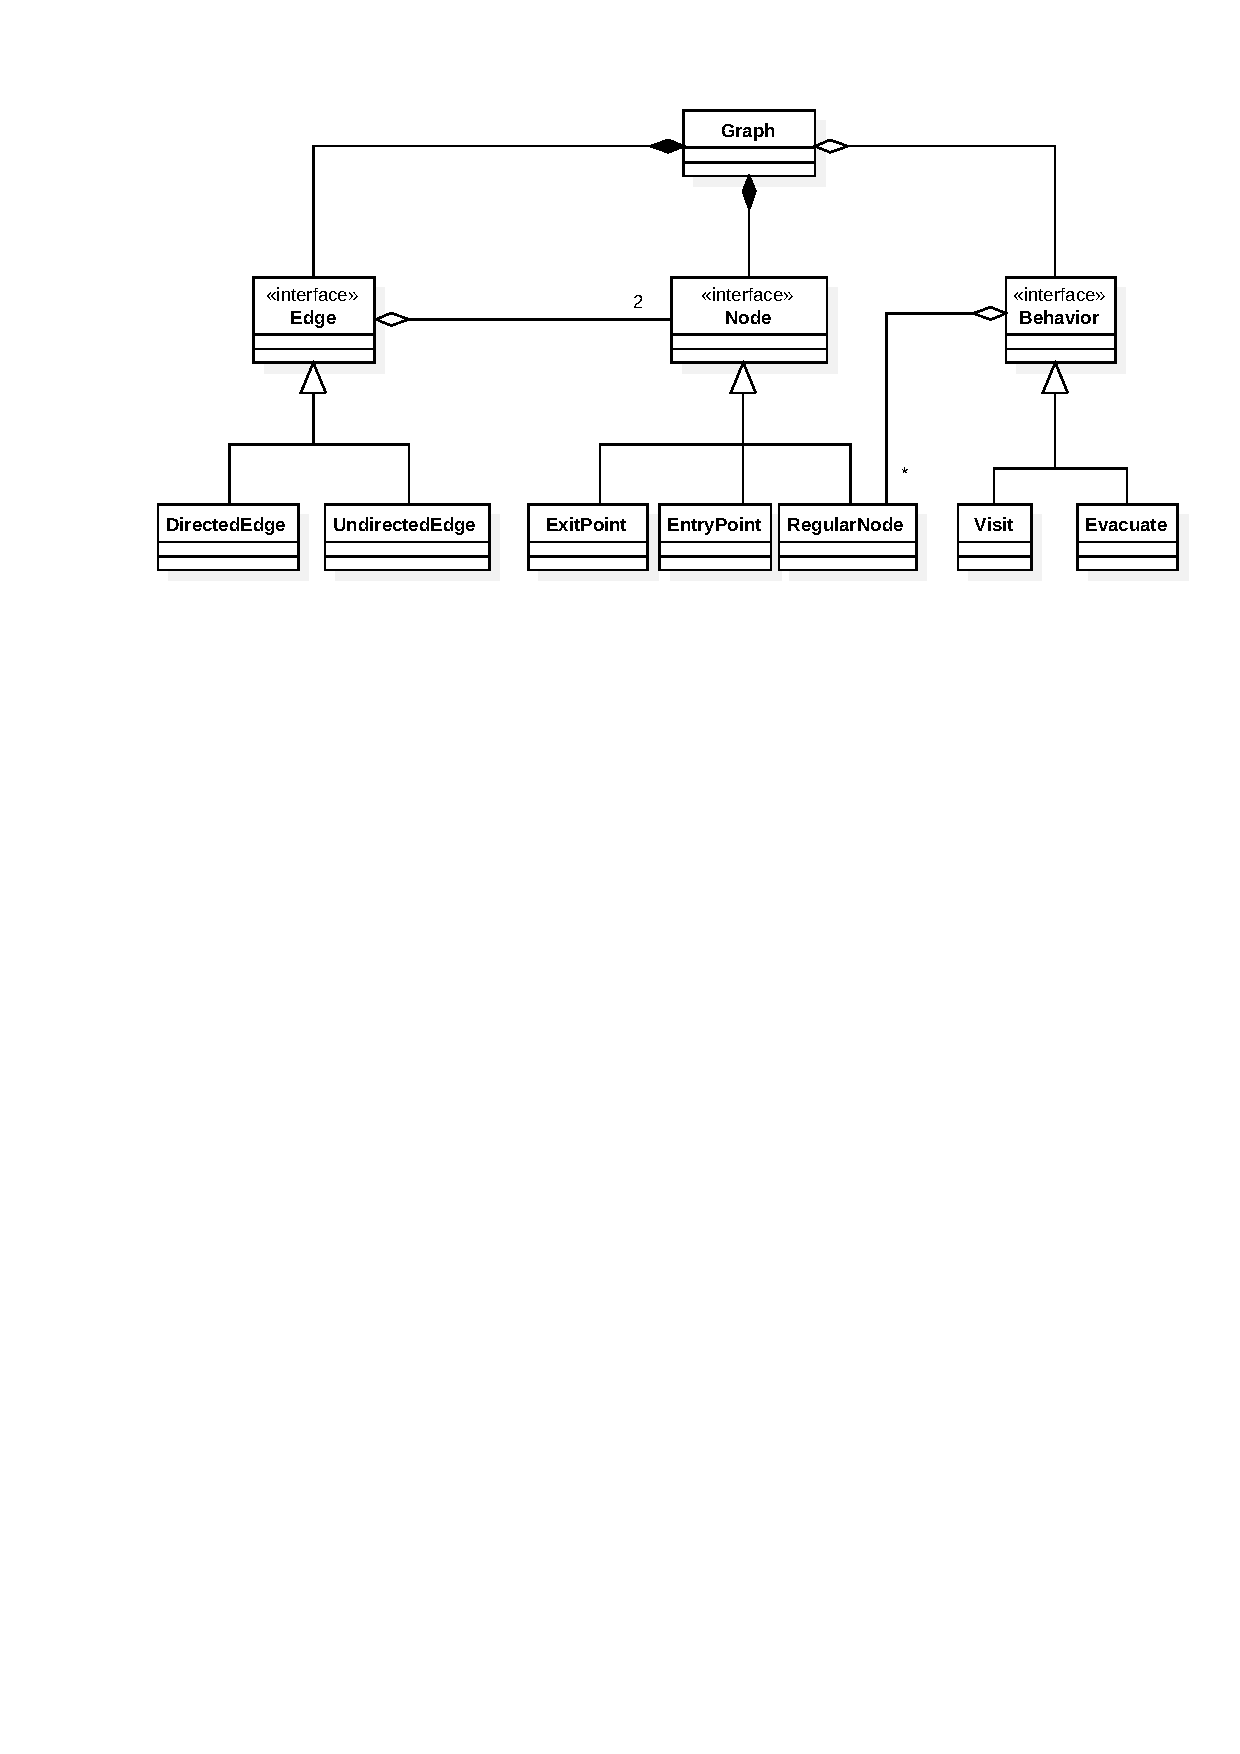
\includegraphics[width=\textwidth,height=\textheight,keepaspectratio]{images/graph-diagram.pdf}
\caption{Class diagram della struttura del grafo}
\label{fig:graph-diagram}
\end{figure}
Ogni behavior è caratterizzato da un identificatore, attribuitogli dall'XML e da una lista di nodi regolari di interesse che devono essere visitati prima di permettere all'attore di puntare ad una uscita. 

\subsection{Parser XML e Builder}
Come già accennato, abbiamo scelto il formato JDOM per la rappresentazione del file XML. La scelta di questo formato è stata dettata dalla sua struttura, che si adatta meglio ai nostri fini di sola lettura e non di manipolazione del documento.\\
\begin{figure}[htbp]
\centering
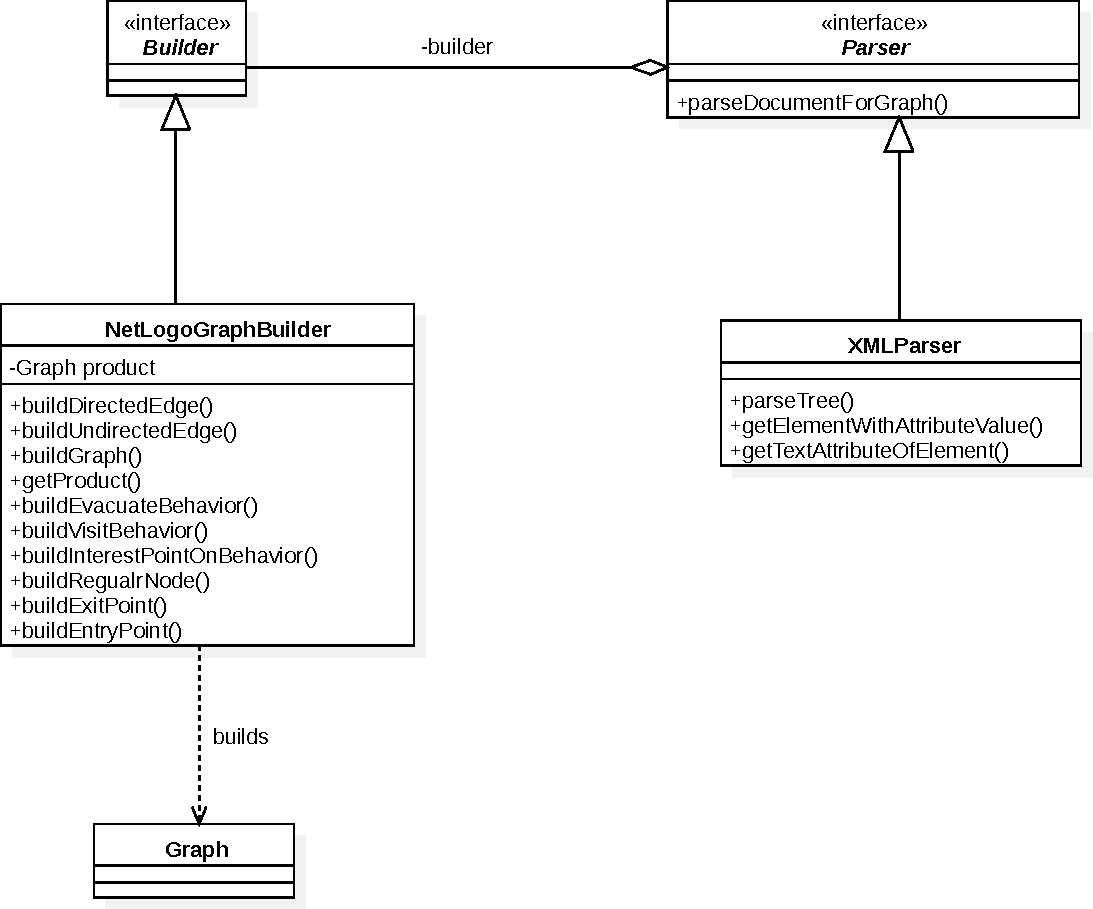
\includegraphics[width=\textwidth,height=\textheight,keepaspectratio]{images/builder-diagram.pdf}
\caption{Class diagram di Parser e Builder}
\label{fig:builder-diagram}
\end{figure}
Per la fase di costruzione delle classi abbiamo usato il pattern Builder, in modo da mantenere il processo di costruzione della struttura interna dell'oggetto di tipo Grafo trasparente all'utente di questo strumento. In particolare l'interfaccia del Builder aiuta a mantenere l'algoritmo di interpretazione dell'XML separato dal processo di costruzione e rappresentazione del suo contenuto in classi Java.\\
Il pattern Builder, inoltre, porta il grande beneficio di migliorare la modularizzazione derivante dall'incapsulamento di tutta la procedura di manipolazione della struttura interna dell'oggetto costruito, in questo modo il Client non ha necessità di conoscere la sua composizione interna.\\
Una conseguenza che rende il pattern ancora più adatto al nostro caso è il miglioramento del controllo sul processo di costruzione del prodotto. Al contrario di altri pattern creazionali, i quali costruiscono e restituiscono il prodotto in un'unica funzione, il Builder separa queste due operazioni mettendo a disposizione un'interfaccia più completa.\\
Grazie a questo noi siamo in grado di esercitare un maggiore controllo sulla correttezza delle operazioni eseguite e delle informazioni inserite durante questa prima fase.\\
L'interfaccia Parser rende il progetto aperto ad estensioni future, come il supporto di linguaggi alternativi al XML.\\
\begin{figure}[htbp]
\centering
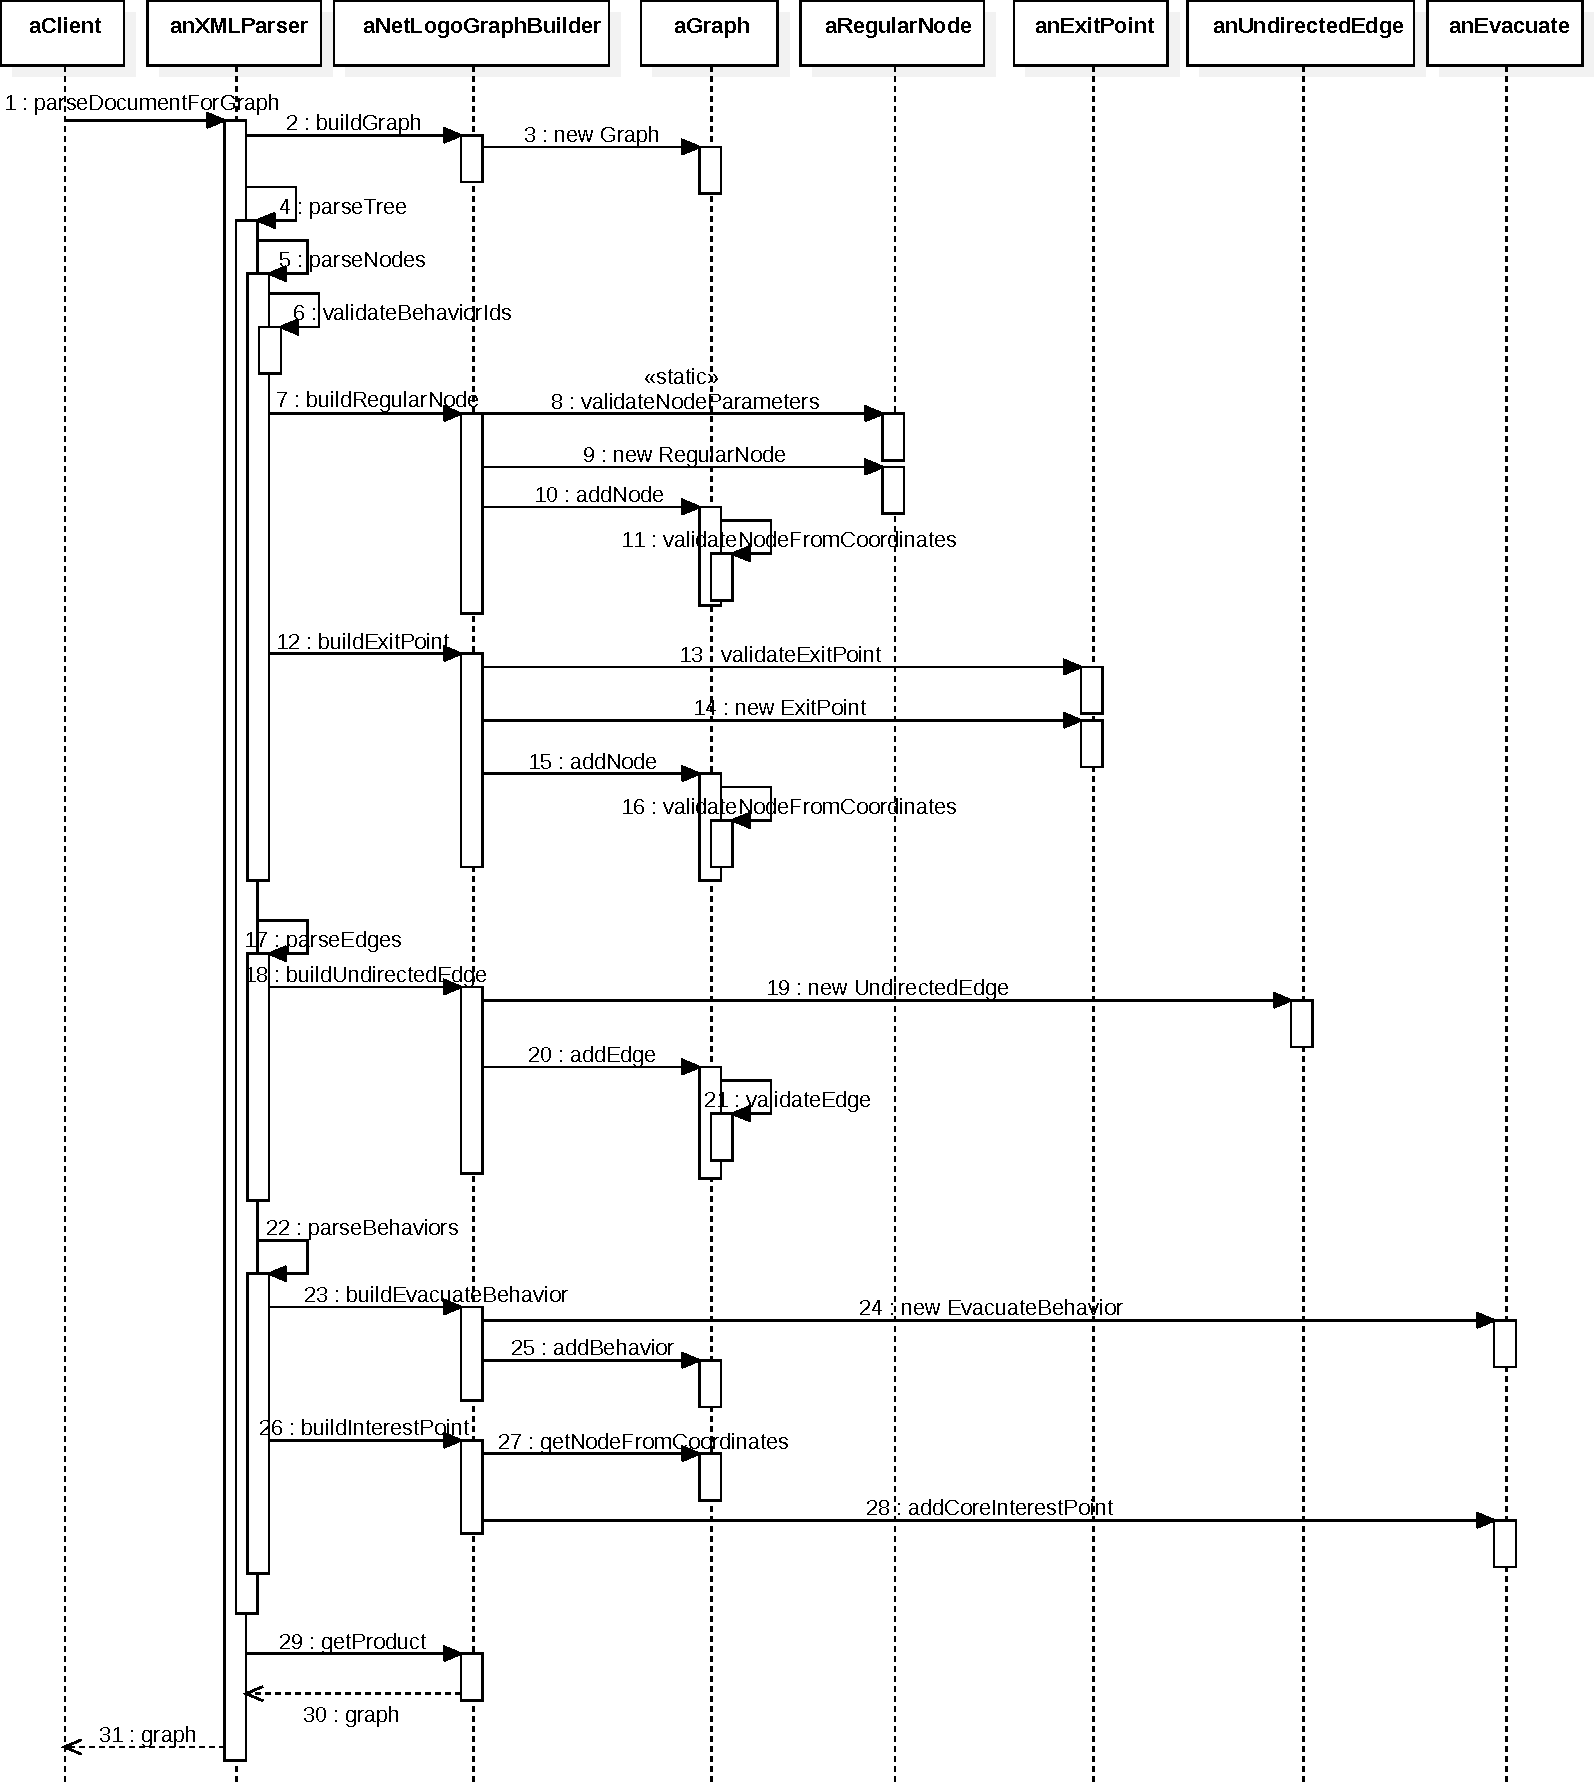
\includegraphics[width=\textwidth,height=\textheight,keepaspectratio]{images/builder-sequence.pdf}
\caption{Sequence diagram della costruzione di un grafo da parte di XMLParser}
\label{fig:builder-sequence}
\end{figure}
Come si vede in Figura \ref{fig:builder-diagram} il parser esercita il ruolo di Director per il builder. Il processo di analisi del documento e costruzione degli oggetti Java è descritto nel sequence diagram in Figura \ref{fig:builder-sequence}.
XMLParser costruisce, attraverso la libreria JDOM2, il modello JDOM del documento, il quale rispecchia la struttura ad albero del documento. Quindi il parser effettua una visita del modello ad albero, legge le informazioni necessarie e impartisce i corretti comandi al builder.\\

\subsection{Visitor}
Per l'operazione di scrittura del codice NetLogo si ha la necessità di estrapolare dagli oggetti che costituiscono la struttura del grafo diverse informazioni. Al variare della classe concreta varieranno anche le informazioni specifiche da estrarre.\\
Il grafo inoltre presenta una struttura di classi con interfacce diverse che devono, quindi, essere modificate per poter eseguire l'operazione necessaria.\\
In questo contesto, quindi, il pattern Visitor si rivela molto utile permettendo di eseguire operazioni specifiche al variare della classe concreta senza inquinare le diverse interfacce all'interno della struttura.\\
Un ulteriore vantaggio presentato dal Visitor è quello di concentrare le funzioni per la scrittura del codice NetLogo in classi specifiche rendendo il sistema più facile da manutenére ed eventualmente estendere.\\
La struttura dei modelli NetLogo finali è tale che gran parte del codice necessario rimane fissa al variare della simulazione, per questo motivo si ha che l'operazione di scrittura del codice NetLogo eseguita dai visitor è alternata a quella di lettura da appositi file di testo che contengono la parte fissa del modello. Queste parti fisse quindi vengono completate con le informazioni estrapolate dagli oggetti Java precedentemente messi in vita.\\
Abbiamo inoltre scelto di separare il modello NetLogo finale in due parti, mantenendo distinta la parte del modello che mette in vita l'ambiente da quella che controlla i movimenti degli attori e raccoglie le informazioni di interesse.\\
\begin{figure}[htb]
\centering
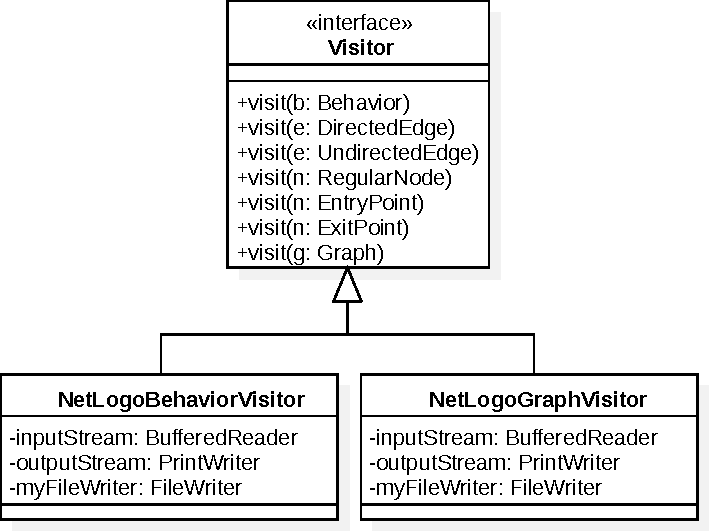
\includegraphics[width=\textwidth,height=\textheight,keepaspectratio]{images/visitor-class-diagram.pdf}
\caption{Class Diagram del Visitor}
\label{fig:visitor-diagram}
\end{figure}
Si hanno quindi due classi visitor distinte per ognuno dei due modelli NetLogo da creare: NetLogoGraphVisitor e NetLogoBehaviorVisitor ( Figura \ref{fig:visitor-diagram} ). Il primo effettua una visitita su nodi e archi del grafo per scrivere i comandi necessari a mettere in vita l'ambiente corretto. Il secondo, invece, effettua una visita sui behaviors in modo da definire i comportamenti che gli attori potranno avere nella simulazione e sui nodi per impostare lo stato iniziale del sistema.\\
In questo modo le interfacce delle classi del grafo, rimangono inalterate ma le operazioni effettuate variano al variare del visitor concreto, rendendolo un pattern ancora più adatto a questo specifico caso.\\
In Figura \ref{fig:visitor-sequence} è mostrato il funzionamento di un NetLogoGraphVisitor. L'oggetto finale ottenuto da questo visitor è un file eseguibile \texttt{.nlogo} in cui viene costruito l'ambiente con la corretta topologia e viene esportato un file di stato del modello nel formato \texttt{.csv} necessario al secondo modello per l'acquisizione dell'ambiente.\\
\begin{figure}[htbp]
\centering
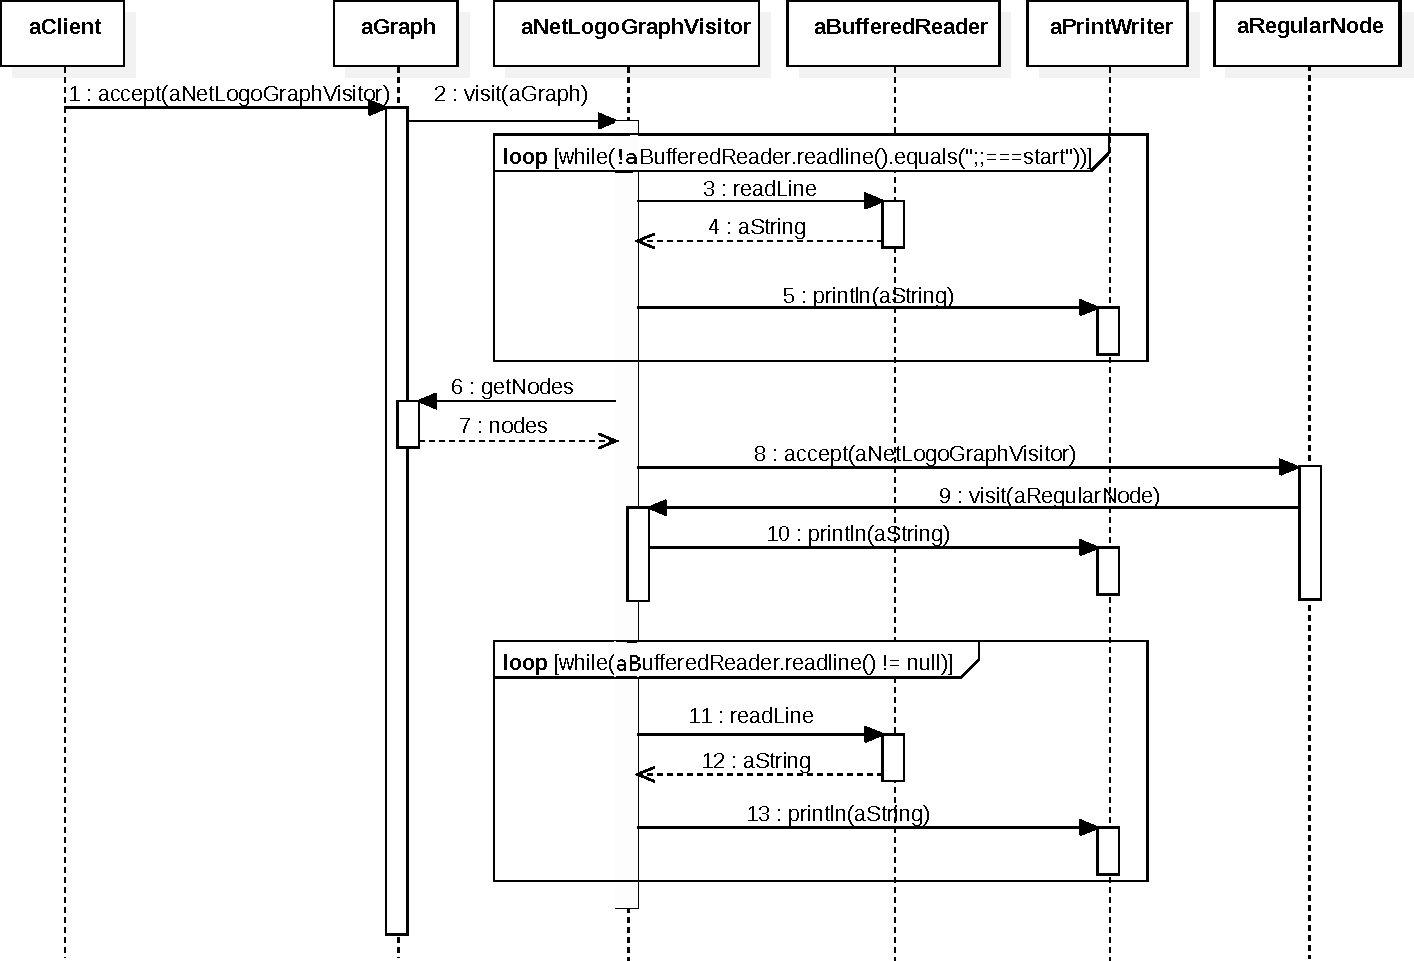
\includegraphics[width=\textwidth,height=\textheight,keepaspectratio]{images/visitor-sequence.pdf}
\caption{Sequence Diagram del NetLogoGraphVisitor su un grafo con un unico nodo}
\label{fig:visitor-sequence}
\end{figure}
NetLogoBehaviorVisitor, in modo analogo, eseguirà operazioni di lettura e scrittura alternate per generare un un secondo file \texttt{.nlogo} in si esegue la simulazione e si esportano i dati di interesse.

\section{Modello NetLogo}
Come già accennato in precedenza abbiamo scelto di dividere il modello NetLogo generato dal nostro programma in due parti con lo scopo di mantenere le funzioni necessarie per la costruzione dell'ambiente separate da quelle che modellano i movimenti degli attori e raccolgono le informazioni sulla simulazione eseguita. In questo modo il codice è più facile da gestire e manutenere.\\
Questa scelta porta, inoltre, il vantaggio di eseguire il primo modello una vola sola e di sfruttare, invece, il file di stato che esso genera nel caso in cui si vogliano simulare le interazioni di diversi comportamenti nello stesso ambiente.
\subsection{Ambiente}
L'ambiente in cui gli attori si muoveranno è modellato sotto forma di grafo con specifiche tipologie di turtles dette \texttt{beacon} che fanno da nodi e rappresentano quindi gli incroci tra le vie percorribili.\\
Gli archi sono rappresentati da due tipologie diverse di turtles dette \texttt{street}, percorribile in entrambi i versi, e \texttt{directed-street}, percorribile solo in un verso.\\
\begin{figure}[htbp]
\centering
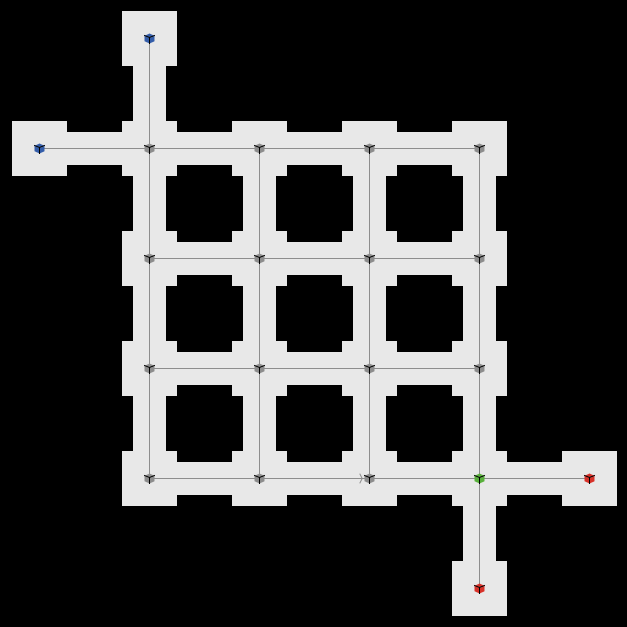
\includegraphics[width=\textwidth,height=\textheight,keepaspectratio]{images/ambiente-screen.png}
\caption{Esempio di ambiente generato. In questo caso i beacons di ingresso sono di colore verde e i beacons di uscita di colore rosso.}
\label{fig:ambiente-screen}
\end{figure}
Per i beacons di ingresso e di uscita vengono anche impostati i relativi parametri, ovvero tasso di generazione o eliminazione degli attori e percentuali relative ai behavior da attribuire ad essi. In particolare per gli entry points si imposta anche un limite massimo del numero di attori che possono essere generati.\\
Grazie a questi parametri il sistema è predisposto per lo studio di simulazioni in ambienti comunicanti, in cui quindi gli attori possono uscire da un ambiente e entrare in un altro. 
\subsection{Behaviors e stato iniziale}
Abbiamo scelto di caratterizzare i behaviors degli attori con un identificatore intero e una lista di nodi di interesse che l'attore deve raggiungere prima di uscire dall'ambiente.\\
Sono state inoltre inserite due possibili modalità di raggiungimento dei beacons di interesse: ”\texttt{minDistance}” e “\texttt{orderedList}”. Nella prima l'attore punta al nodo più vicino a quello precedentemente raggiunto tra quelli di interesse, nella seconda invece la lista viene rigidamente percorsa rispettandone l'ordine.\\
Lo stato iniziale del sistema è contenuto in una semplice lista \texttt{initial-state} che viene percorsa da una apposita funzione per la corretta generazione degli attori sui vari nodi. 
\begin{figure}[htbp]
\centering
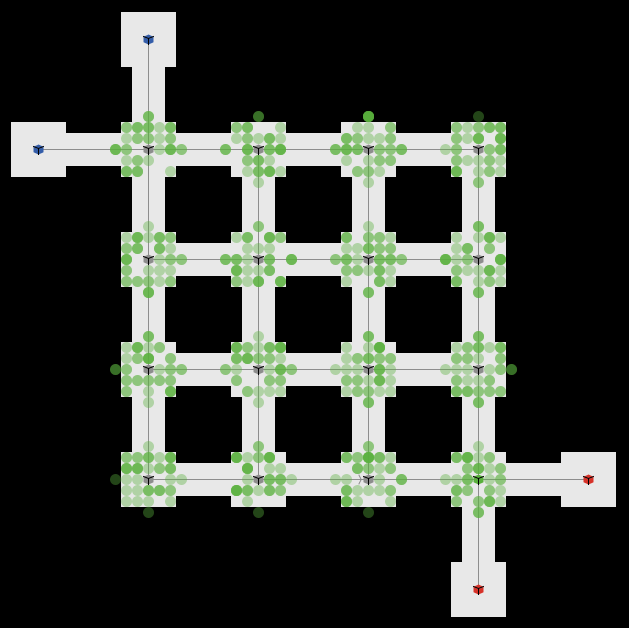
\includegraphics[width=\textwidth,height=\textheight,keepaspectratio]{images/movers-screen.png}
\caption{Esempio di ambiente popolato con attori nello stato iniziale. Gli attori hanno assunto il colore del beacon che hanno come obiettivo, in questo caso abbiamo un unico behavior che ha come interest point il beacon di colore rosa.}
\label{fig:movers-screen}
\end{figure}

\begin{figure}[htbp]
\centering
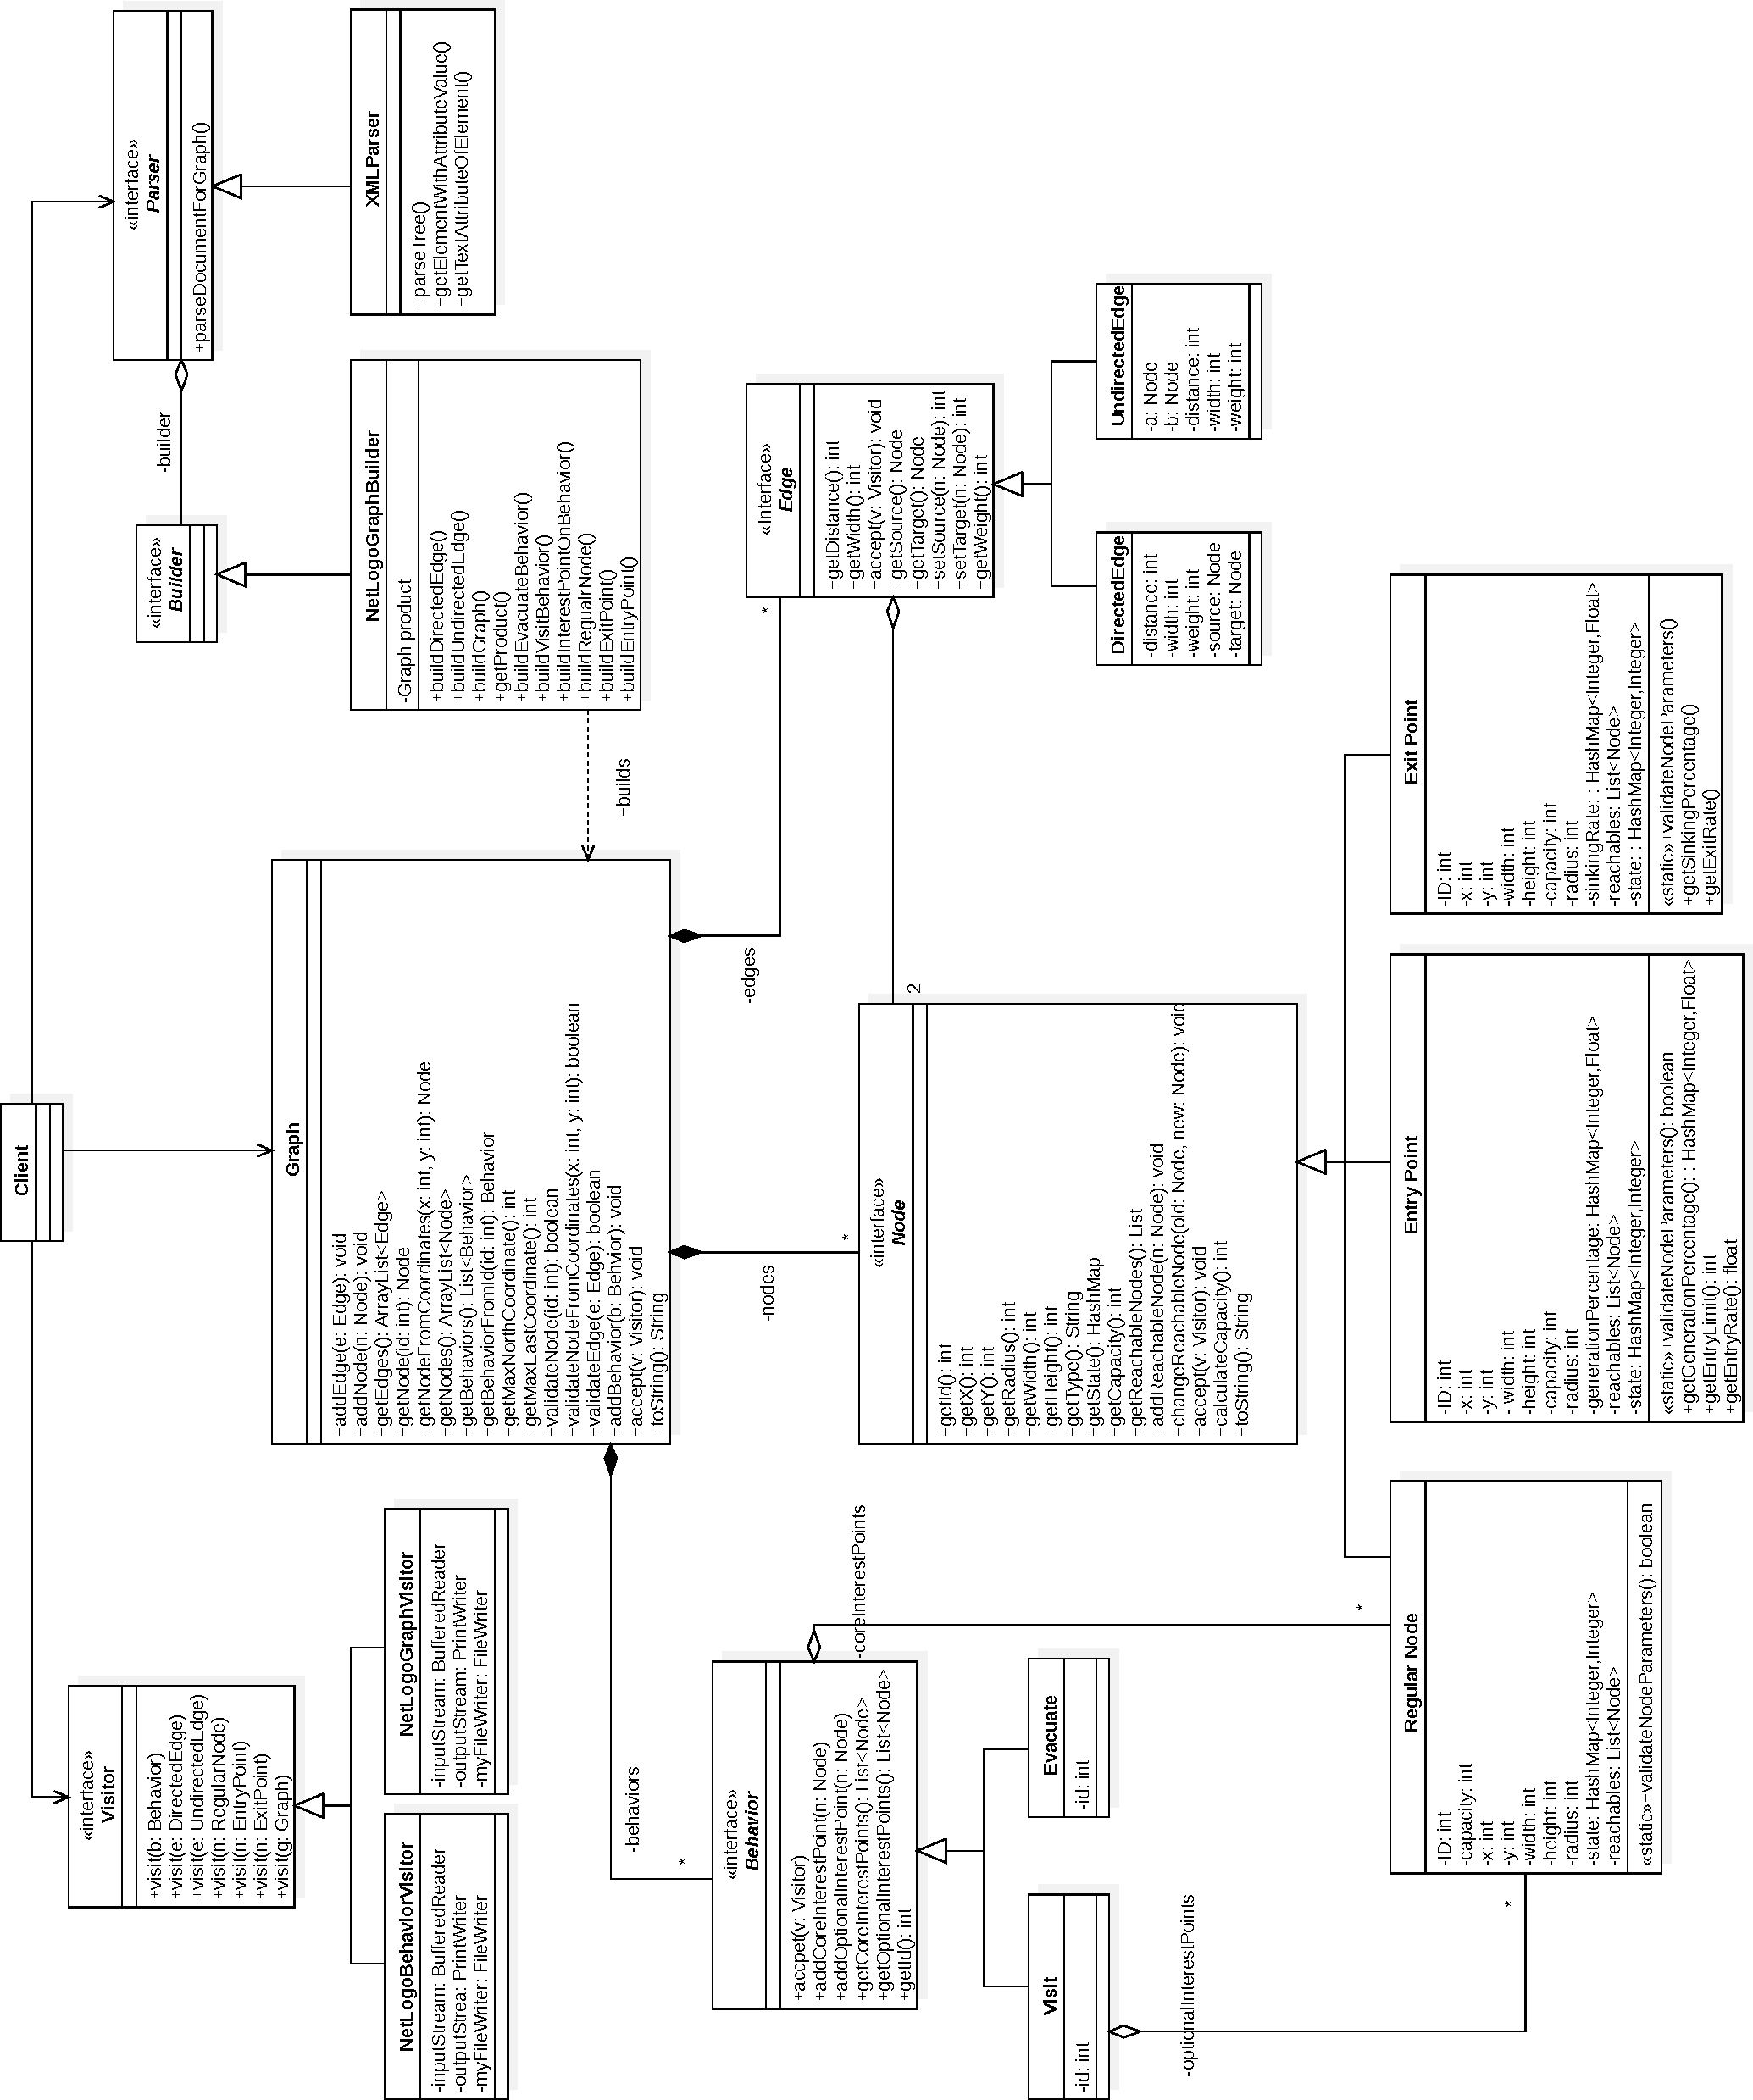
\includegraphics[width=\textwidth,height=\textheight,keepaspectratio]{images/complete-diagram.pdf}
\caption{Classi diagram}
\label{fig:complete-diagram}
\end{figure}
%\chapter{Sviluppo del progetto}
\label{cap:sviluppo-progetto}

L'obiettivo di questa tesi è realizzare un programma in linguaggio Java che sia in grado di ricevere in ingresso la struttura del modello descritta in linguaggio XML e di scrivere in modo automatico il codice NetLogo che possa eseguire la simulazione di interesse, rendendo, quindi, trasparente il processo di scrittura del codice.

Questo progetto è costituito da una struttura composita centrale di classi in cui vengono conservate tutte le informazioni necessarie per l'esecuzione della simulazione. Come mostrato nella Sezione \ref{sec:strttura-interna} l'oggetto di tipo Graph che rappresenta la struttura è composto da classi che modellano la topologia dell'ambiente e da classi che rappresentano i comportamenti da simulare.

L'informazione conservata in questa struttura viene estratta da un apposito parser che implementa il pattern Builder per la costruzione e composizione degli oggetti.

Infine si è implementato il pattern Visitor per visitare gli oggetti della struttura e generare il relativo codice NetLogo.

I modelli NetLogo che vengono generati da questo componente sono costituiti da un ambiente fisico modellato sotto forma di grafo con nodi e archi che rappresentano rispettivamente incroci e strade, caratterizzati da coordinate spaziali e dimensioni fisiche. In questo ambiente si muovono attori che possono avere comportamenti differenti. Nel nostro caso abbiamo deciso di modellare i comportamenti degli attori come una lista di punti di interesse che questi devono visitare prima di poter uscire.

Nella Sezione \ref{sec:doc-xml} andiamo a delineare la struttura dei documenti XML previsti e nella Sezione \ref{subsec:parser-builder} si descrive brevemente il funzionamento del relativo parse. Nella Sezione \ref{sec:modello-netlogo} invece tracciamo la struttura del modelli NetLogo generati. Infine nella Sezione \ref{sec:librerie} si descrivono le librerie usate.

\section{Struttura centrale}
\label{sec:strttura-interna}

L'unico scopo delle classi Java utilizzate è quello di rappresentare e conservare l'informazione raccolta dal documento XML, senza eseguire alcun tipo di manipolazione. Per questo motivo abbiamo cercato di mantenere la struttura delle classi il più semplice possibile, come mostrato in Figura \ref{fig:graph-diagram}.

La classe Graph è caratterizzata da una composizione di Edge, Node e Behavior. Espone metodi per il recupero delle informazioni e per la validazione di nodi e archi, in modo tale da impedire l'aggiunta di nodi nella medesima posizione e di archi con gli estremi uguali.

\begin{figure}[htbp]
\centering
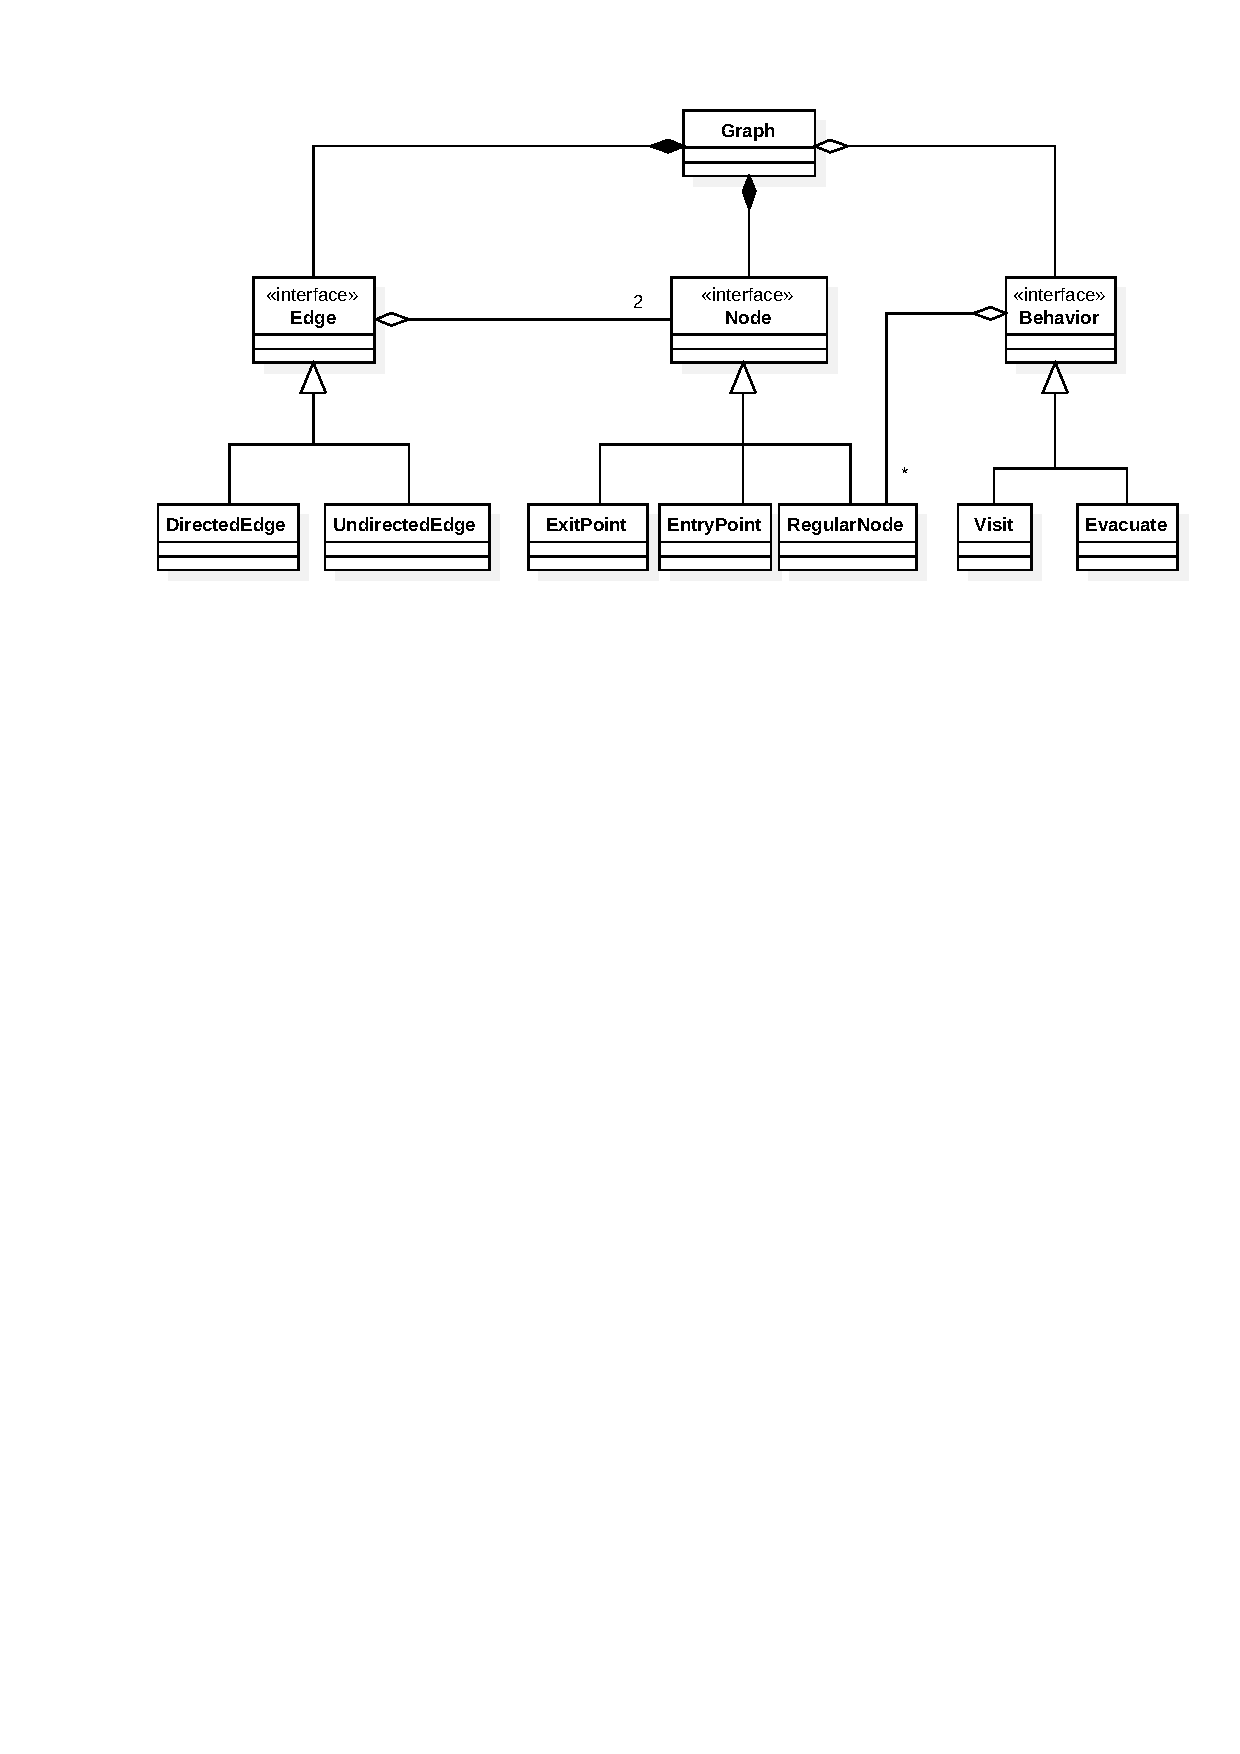
\includegraphics[width=\textwidth,height=\textheight,keepaspectratio]{images/graph-diagram.pdf}
\caption{Class diagram della struttura del grafo}
\label{fig:graph-diagram}
\end{figure}
Ogni behavior è caratterizzato da un identificatore, attribuitogli dall'XML e da una lista di nodi regolari di interesse che devono essere visitati prima di permettere all'attore di puntare ad una uscita.

Gli edges in questo modello sono aggregazioni di due nodi e presentano un particolare attributo “weight” che verrà usato dalle funzioni NetLogo per la generazione dei percorsi a costo minimo.

Infine ogni classe che implementa l'interfaccia Node, oltre ai metodi per il recupero delle informazioni conservate, implementa anche un metodo statico per il controllo dei parametri, in modo tale da impedire la costruzione di nodi con informazioni incompatibili con NetLogo.

%
\begin{figure}[htbp]
\centering
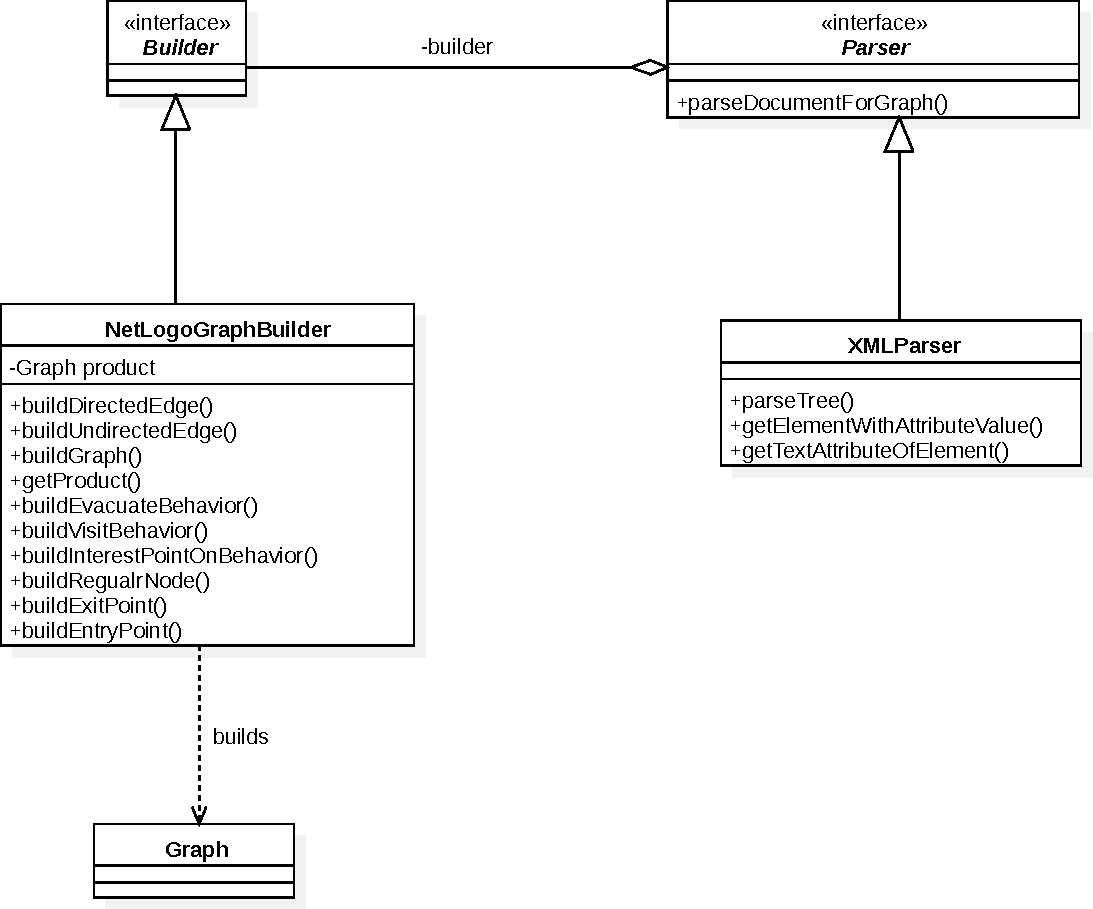
\includegraphics[width=\textwidth,height=\textheight,keepaspectratio]{images/builder-diagram.pdf}
\caption{Class diagram di Parser e Builder}
\label{fig:builder-diagram}
\end{figure}
\section{Builder}
\label{sec:builder}
Per la costruzione delle classi abbiamo usato il pattern Builder, in modo da mantenere il processo di costruzione della struttura interna dell'oggetto di tipo Grafo trasparente all'utente di questo strumento. In particolare l'interfaccia del Builder aiuta a mantenere l'algoritmo di interpretazione dell'XML separato dal processo di costruzione e rappresentazione del suo contenuto in classi Java.

Il pattern Builder, inoltre, porta il grande beneficio di migliorare la modularizzazione derivante dall'incapsulamento di tutta la procedura di manipolazione della struttura interna dell'oggetto costruito, in questo modo il Client non ha necessità di conoscere la sua composizione interna.

Una conseguenza che rende il pattern ancora più adatto al nostro caso è il miglioramento del controllo sul processo di costruzione del prodotto. Al contrario di altri pattern creazionali, i quali costruiscono e restituiscono il prodotto in un'unica funzione, il Builder separa queste due operazioni mettendo a disposizione un'interfaccia più completa.

Grazie a questo noi siamo in grado di esercitare un maggiore controllo sulla correttezza delle operazioni eseguite e delle informazioni inserite durante questa prima fase.

L'interfaccia Parser rende il progetto aperto ad estensioni future, come il supporto di linguaggi alternativi all'XML.

\begin{figure}[htbp]
\centering
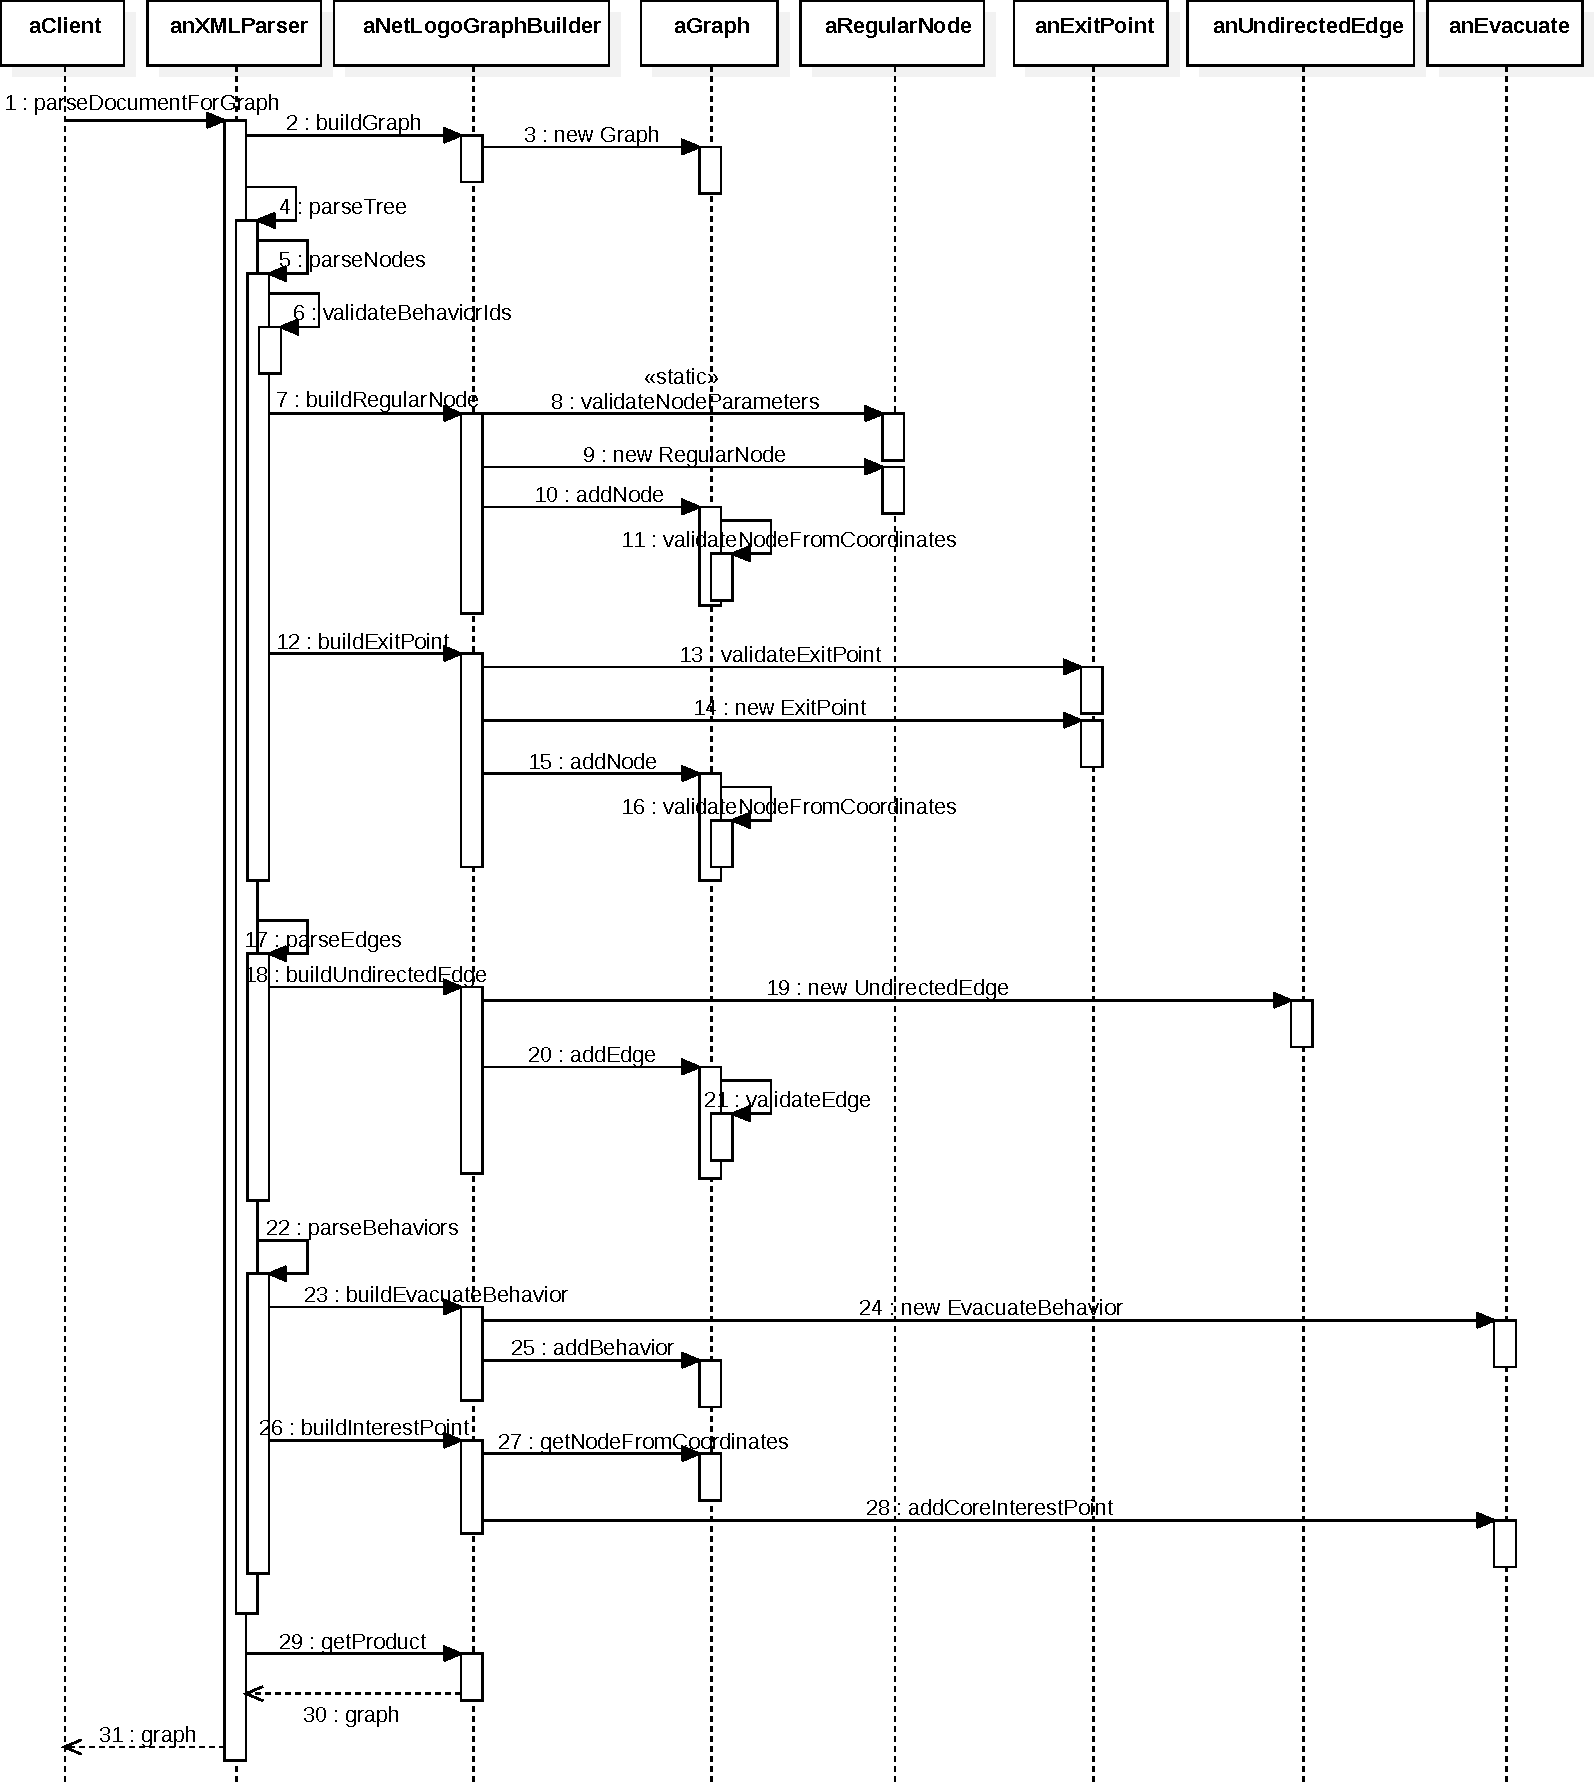
\includegraphics[width=\textwidth,height=\textheight,keepaspectratio]{images/builder-sequence.pdf}
\caption{Sequence diagram della costruzione di un grafo da parte di XMLParser}
\label{fig:builder-sequence}
\end{figure}

In Figura \ref{fig:builder-diagram} si può osservare la struttura delle classi che implementano questo pattern.

\subsection{Funzionamento}
La classe \texttt{XMLParser} svolge il ruolo di \textit{Director} all'interno del pattern e, durante la visita della struttura JDOM \cite{jdom} creata, chiama i metodi del \textit{ConcreteBuilder} \texttt{NetLogoGraphBuilder} per la costruzione dei vari oggetti e la loro composizione a formare la struttura centrale.

Quando la visita da parte del parser è conclusa viene recuperato il \textit{Product}, che non è altro che un oggetto di tipo \texttt{Graph}, in Figura \ref{fig:builder-sequence} si può seguire il processo di costruzione di un semplice modello.

Come prima cosa vengono costruite le classi relative ai nodi, \texttt{XMLParser} estrae le informazioni dalla struttura JDOM e controlla che non vi siano mancanze, quindi chiama lo specifico metodo di costruzione del builder.

Il \texttt{NetLogoGraphBuilder}, prima di procedere alla messa in vita dell'oggetto, verifica, tramite un metodo statico della relativa classe, che le informazioni da inserire siano corrette, ad esempio si controlla che le dimensioni fisiche dell'incrocio non siano negative. Una volta costruito l'oggetto il builder chiama la funzione della classe \texttt{Graph} per aggiungere il nodo alla struttura, questa operazione è preceduta da un controllo sui nodi già presenti per evitare sovrapposizioni.

In modo analogo vengono costruiti e aggiunti alla struttura anche gli archi. Si costruisce l'arco e si delega a \texttt{Graph} la responsabilità di evitare l'inserimento di grafi con estremi uguali.

Infine si costruiscono i behaviors sui quali poi si aggiungono i riferimenti ai nodi di interesse sfruttando i metodi esposti dalla classe \texttt{Graph}.

L'operazione finale eseguita dal \texttt{NetLogoGraphBuilder} è quella di restituzione del prodotto costruito tramite il metodo \texttt{getProduct()}.

\section{Visitor}
\label{subsec:visitor}
Per l'operazione di scrittura del codice NetLogo si ha la necessità di estrapolare dagli oggetti che costituiscono la struttura del grafo diverse informazioni. Al variare della classe concreta varieranno anche le informazioni specifiche da estrarre.

Il grafo inoltre presenta una struttura di classi con interfacce diverse che devono, quindi, essere modificate per poter eseguire l'operazione necessaria.

In questo contesto, quindi, il pattern Visitor si rivela molto utile permettendo di eseguire operazioni specifiche al variare della classe concreta senza inquinare le diverse interfacce all'interno della struttura.

Un ulteriore vantaggio presentato dal Visitor è quello di concentrare le funzioni per la scrittura del codice NetLogo in classi specifiche rendendo il sistema più facile da manutenére ed eventualmente estendere.

La struttura dei modelli NetLogo finali è tale che gran parte del codice necessario rimane fissa al variare della simulazione, per questo motivo si ha che l'operazione di scrittura del codice NetLogo eseguita dai visitor è alternata a quella di lettura da appositi file di testo che contengono la parte fissa del modello. Queste parti fisse quindi vengono completate con le informazioni estrapolate dagli oggetti Java precedentemente messi in vita.

Abbiamo inoltre scelto di separare il modello NetLogo finale in due parti, mantenendo distinta la parte del modello che mette in vita l'ambiente da quella che controlla i movimenti degli attori e raccoglie le informazioni di interesse.

\begin{figure}[htb]
\centering
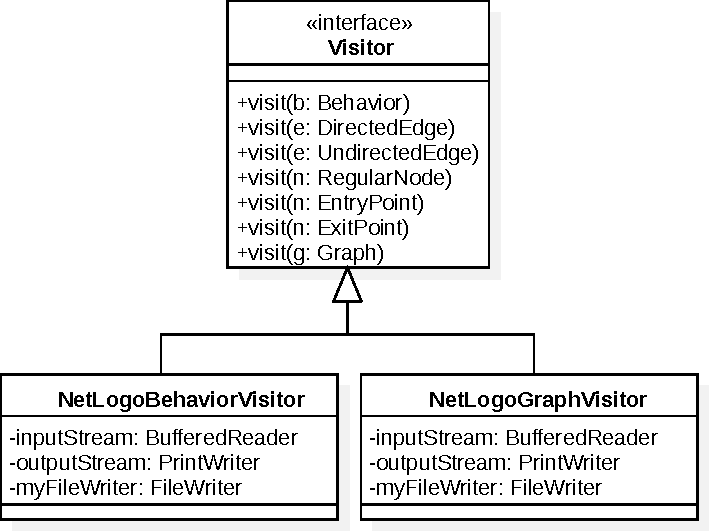
\includegraphics[width=\textwidth,height=\textheight,keepaspectratio]{images/visitor-class-diagram.pdf}
\caption{Class Diagram del Visitor}
\label{fig:visitor-diagram}
\end{figure}
Si hanno quindi due classi visitor distinte per ognuno dei due modelli NetLogo da creare: \texttt{NetLogoGraphVisitor} e \texttt{NetLogoBehaviorVisitor} ( Figura \ref{fig:visitor-diagram} ). Il primo effettua una visitita su nodi e archi del grafo per scrivere i comandi necessari a mettere in vita l'ambiente corretto. Il secondo, invece, effettua una visita sui behaviors in modo da definire i comportamenti che gli attori potranno avere nella simulazione e sui nodi per impostare lo stato iniziale del sistema.

In questo modo le interfacce delle classi del grafo, rimangono inalterate ma le operazioni effettuate variano al variare del visitor concreto, rendendolo un pattern ancora più adatto a questo specifico caso.

\begin{figure}[htbp]
\centering
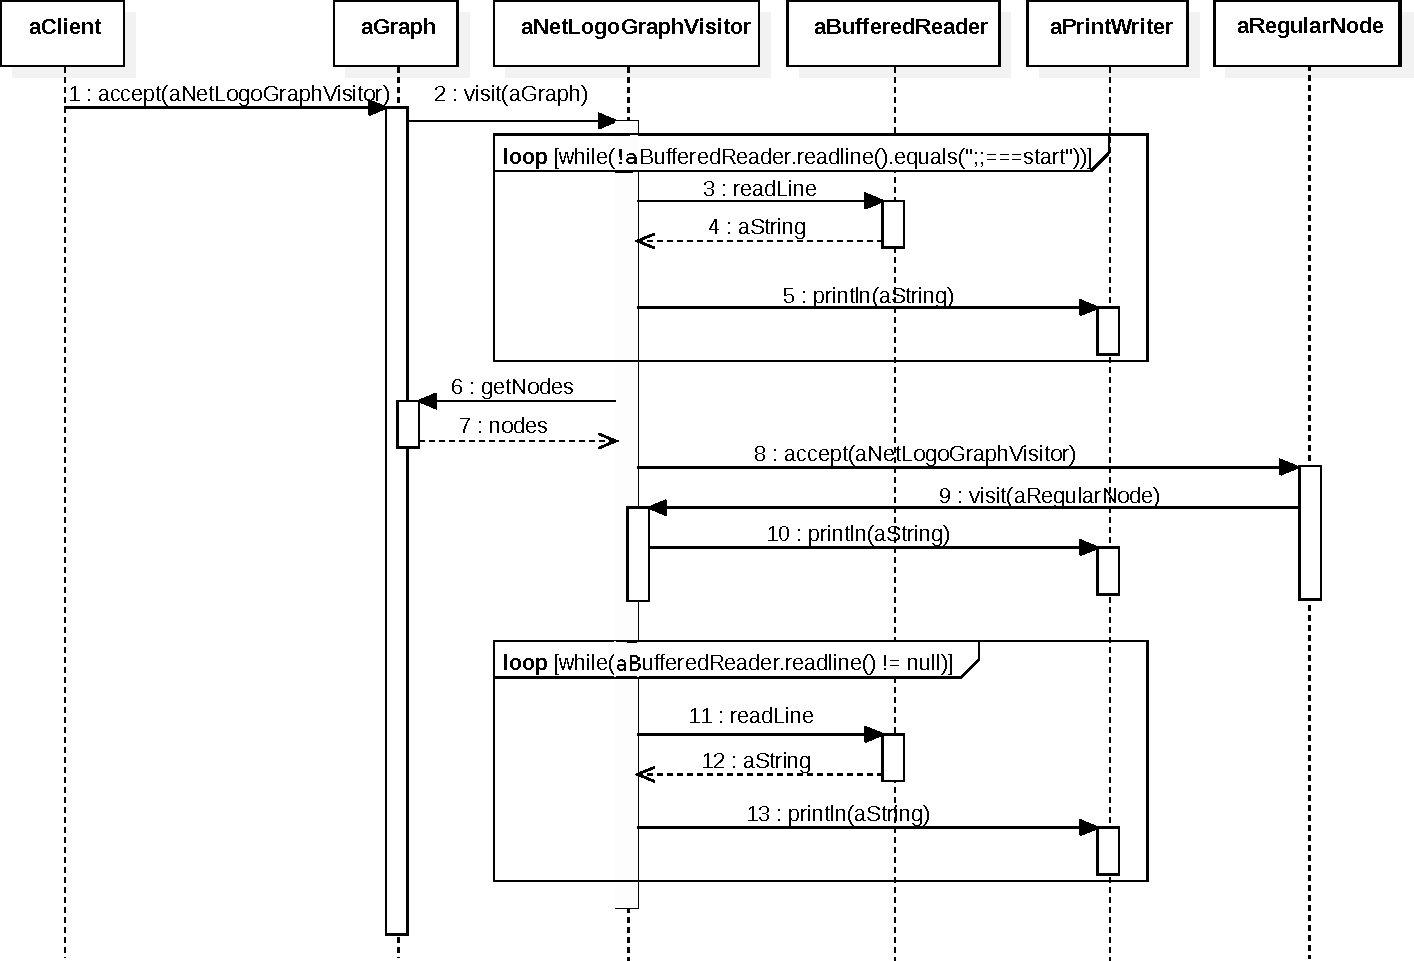
\includegraphics[width=\textwidth,height=\textheight,keepaspectratio]{images/visitor-sequence.pdf}
\caption{Sequence Diagram del NetLogoGraphVisitor su un grafo con un unico nodo}
\label{fig:visitor-sequence}
\end{figure}
NetLogoBehaviorVisitor, in modo analogo, eseguirà operazioni di lettura e scrittura alternate per generare un un secondo file \texttt{.nlogo} in cui si esegue la simulazione e si esportano i dati di interesse.

\subsection{Funzionamento}
In Figura \ref{fig:visitor-sequence} è mostrato il funzionamento di un \texttt{NetLogoGraphVisitor}.Come prima cosa si trascrive una parte del codice contenuto nel file di testo fino alla specifica stringa di flag “\texttt{;;===start}”.

Quindi vengono estratte dal grafo informazioni riguardanti le dimensioni globali dell'ambiente che deve essere generato e vengono scritte le relative procedure NetLogo per la sua impostazione.

Il visitor estrae dal grafo le liste dei nodi e degli archi che lo costituiscono e procede alla loro visita.

Trattandosi del visitor per la generazione dell'ambiente fisico, vengono estratte solo le informazioni riguardanti le dimensioni fisiche delle entità rappresentate dagli oggetti. In particolare per i nodi di ingresso e uscita vengono anche impostate le variabili relative al tasso di generazione o eliminazione e le liste sulle percentuali relative ad ogni behavior. Si noti che questo visitor non aggiunge alcun tipo di funzionalità alle classi che rappresentano i comportamenti.

In modo analogo \texttt{NetLogoBehaviorVisitor} trascrive parte del codice dal file di testo fino ad arrivare alla stringa “\texttt{;;===behaviors}”.\\
Il visitor quindi esegue una visita su tutti i behaviors presenti nel modello Java andando a scrivere in NetLogo le procedure per la creazione di una apposita tabella in cui si indicizzano tutti i comportamenti con i loro punti di interesse.

A questo punto si trascrive un'altra porzione di codice dal file di testo fino ad arrivare alla stringa “\texttt{;;===system}” che indica il punto all'interno del file in cui devono essere inserite le procedure per l'impostazione dello stato iniziale.

Vengono visitati nuovamente tutti i nodi da cui, ora, si estraggono informazioni sulla quantità di attori presenti e i loro comportamenti. Queste informazioni vengono usate dal visitor per popolare una specifica lista del modello NetLogo in cui si è conservato lo stato. Anche in questo caso, si può osservare che \texttt{NetLogoBehaviorVisitor} non aggiunge funzionalità agli archi del grafo. 

\section{Documento XML}
\label{sec:doc-xml}

\definecolor{darkgreen}{rgb}{0,0.5,0}

\lstdefinelanguage{XML}{
  basicstyle=\linespread{0.9}\ttfamily,
  morestring=[s]{"}{"},
  morecomment=[s]{!--}{--},
  commentstyle=\color{blue},
  moredelim=[s][\color{black}]{>}{<},
  moredelim=[s][\color{violet}]{\ }{=},
  stringstyle=\color{red},
  identifierstyle=\color{darkgreen},
  tabsize=2,
  breaklines=true,
  breakatwhitespace=true
}

La struttura del documento XML prevista per il funzionamento del nostro strumento si attiene il più possibile allo standard di formato GraphML \cite{graphml} (approvato dal W3C) in modo da evitare inconsistenze e incomprensioni, soprattutto per la parte in cui è descritta la topologia dell'ambiente, per la quale questo formato è pienamente adatto. Il file XML è suddiviso in tre sezioni distinte: \texttt{Graph}, \texttt{Behaviors}, \texttt{System}.

\subsection{Graph} 

Rappresenta la topologia dell'ambiente in cui gli attori si muovono, ed è descritta sotto forma di grafo con \texttt{edges} che rappresentano le strade e \texttt{nodes} che rappresentano gli incroci.

Gli edges possono essere \texttt{directed} e \texttt{undirected}, per ognuno di essi vengono specificati peso e larghezza, ovvero \texttt{weight} e \texttt{eWidth} come mostrato in Figura \ref{fig:xml-edges}. Il formato GraphML, inoltre, permette di specificare un tipo di default per gli edges come valore dell'attributo \texttt{edgedefault} di Graph.

\begin{figure}[htbp]
\centering
\lstinputlisting[language=XML, firstline=178, lastline=188]{images/example.xml} %edges
\caption{Esempio XML di definizione delle due tipologie di archi}
\label{fig:xml-edges}
\end{figure}

I nodes invece possono essere di tre tipi: normal, entry o exit. Per tutti e tre i tipi vengono specificate coordinate spaziali e dimensioni fisiche dell'incrocio che esso rappresenta, quindi avremo \texttt{nx}, \texttt{ny}, \texttt{nWidth}, \texttt{nHeight} e \texttt{nRadius}. All'interno del codice si usa l'attributo \texttt{nType} per specificare il tipo di nodo e anche in questo caso è possibile specificare un tipo di default settato a \texttt{normal}. In Figura \ref{fig:xml-nodes} mostriamo un esempio della definizione delle tre tipologie di nodi.  

\begin{figure}[htbp]
\centering
\lstinputlisting[language=XML, firstline=32, lastline=38]{images/example.xml} %nodo regolare
\lstinputlisting[language=XML, firstline=152, lastline=169]{images/example.xml} %entry e exit node
\caption{Esempio XML di definizione delle tre tipologie di nodi}
\label{fig:xml-nodes}
\end{figure}


\subsection{Behaviors}

Per quanto riguarda i \texttt{Behaviors} si ha una struttura a grafo, mostrata in Figura \ref{fig:xml-behaviors}, in cui ogni nodo rappresenta un behavior di cui viene indicata la tipologia, ovvero \texttt{bType}, l'identificatore e la lista dei nodi di interesse.

\begin{figure}[htbp]
\centering
\lstinputlisting[language=XML, firstline=299, lastline=308]{images/example.xml} %behavior 
\caption{Esempio XML di definizione di un behavior}
\label{fig:xml-behaviors}
\end{figure}

\subsection{System}

La sezione \texttt{System} descrive lo stato iniziale dell'ambiente. Per questa parte del modello si è preferito distaccarci leggermente dallo standard, in modo da avere una struttura più comprensibile, usando gli specifici tag \texttt{<behavior \textbackslash>}. In Figura \ref{fig:xml-system} si può osservare che per ogni nodo, sotto il tag “\texttt{graph}” con identificatore \texttt{state}, viene indicato il comportamento e la quantità degli attori presenti. In particolare, nei nodi contrassegnati come entry o exit, vi è un ulteriore tag “\texttt{graph}” con identificatore \texttt{parameters} in cui si specificano la frequenza di generazione o eliminazione degli attori e le percentuali relative ad ogni behavior. Per i nodi di ingresso viene anche indicato un limite superiore agli attori generabili (\texttt{entry-limit}), che può essere messo negativo nel caso in cui, invece, non si vogliano porre limiti.

\begin{figure}[htbp]
\centering
\lstinputlisting[language=XML, firstline=310, lastline=318]{images/example.xml} %stato nodo regolare
\lstinputlisting[language=XML, firstline=439, lastline=469]{images/example.xml} %stato entry e exit
\lstinputlisting[language=XML, firstline=484, lastline=485]{images/example.xml} %chiusura tag
\caption{Esempio XML di definizione dello stato iniziale per ogni tipologia di nodo}
\label{fig:xml-system}
\end{figure}

%\subsection{Esempio}
%Di seguito è riportato un XML in cui si mostra la definizione di ogni tipo di entità coinvolta: attributi, tutti i tipi di nodi, tutti i tipi di archi, behavior e stato associato ai nodi.
%
%
%\lstinputlisting[language=XML, firstline=0, lastline=6]{images/example.xml} %attributi
%\[\texttt{[...]}\]
%\lstinputlisting[language=XML, firstline=30, lastline=38]{images/example.xml} %nodo regolare
%\[\textbf{[...]}\]
%\lstinputlisting[language=XML, firstline=152, lastline=169]{images/example.xml} %entry e exit node
%\[\textbf{[...]}\]
%\lstinputlisting[language=XML, firstline=178, lastline=188]{images/example.xml} %edges
%\[\textbf{[...]}\]
%\lstinputlisting[language=XML, firstline=297, lastline=297]{images/example.xml} %chiusa graph
%
%
%\lstinputlisting[language=XML, firstline=299, lastline=308]{images/example.xml} %behavior 
%
%
%\lstinputlisting[language=XML, firstline=310, lastline=318]{images/example.xml} %stato nodo regolare
%\[\textbf{[...]}\]
%\lstinputlisting[language=XML, firstline=439, lastline=469]{images/example.xml} %stato entry e exit
%\[\textbf{[...]}\]
%\lstinputlisting[language=XML, firstline=484, lastline=485]{images/example.xml} %chiusura tag

\section{Parser XML}
\label{subsec:parser-builder}

Come come verrà spiegato nella Sezione \ref{sec:librerie}, abbiamo scelto il formato JDOM per la rappresentazione del file XML. La scelta di questo formato è stata dettata dalla sua struttura, che si adatta meglio ai nostri fini di sola lettura e non di manipolazione del documento.

La struttura ad albero del modello generato rispecchia il documento XML. Ogni nodo dell'albero è di tipo \texttt{Element} e conserva una lista dei figli e un riferimento al padre, espone inoltre una ricca interfaccia con cui si possono estrarre tutte le informazioni di interesse come gli attributi associati al tag rappresentato, oppure il testo sottostante.

Il parser XML inoltre esegue controlli mirati a verificare che siano fornite tutte le informazioni necessarie all'esecuzione del modello NetLogo, ad esempio controlla che per ogni nodo sia specificato lo stato iniziale, compresi parametri come tasso di generazione o eliminazione per nodi di ingresso o uscita.


\section{Modello NetLogo}
\label{sec:modello-netlogo}

Come già accennato in precedenza abbiamo scelto di dividere il modello NetLogo generato dal nostro programma in due parti con lo scopo di mantenere le funzioni necessarie per la costruzione dell'ambiente separate da quelle che modellano i movimenti degli attori e raccolgono le informazioni sulla simulazione eseguita. In questo modo il codice è più facile da gestire e manutenere.

Questa scelta porta, inoltre, il vantaggio di eseguire il primo modello una vola sola e di sfruttare, invece, il file di stato che esso genera nel caso in cui si vogliano simulare le interazioni di diversi comportamenti nello stesso ambiente.
\subsection{Ambiente}
L'ambiente in cui gli attori si muoveranno è modellato sotto forma di grafo con specifiche tipologie di turtles dette \texttt{beacons} che fanno da nodi e rappresentano quindi gli incroci tra le vie percorribili.

Gli archi sono rappresentati da due tipologie diverse di turtles dette \texttt{streets}, percorribili in entrambi i versi, e \texttt{directed-streets}, percorribili solo in un verso.

\begin{figure}[htbp]
\centering
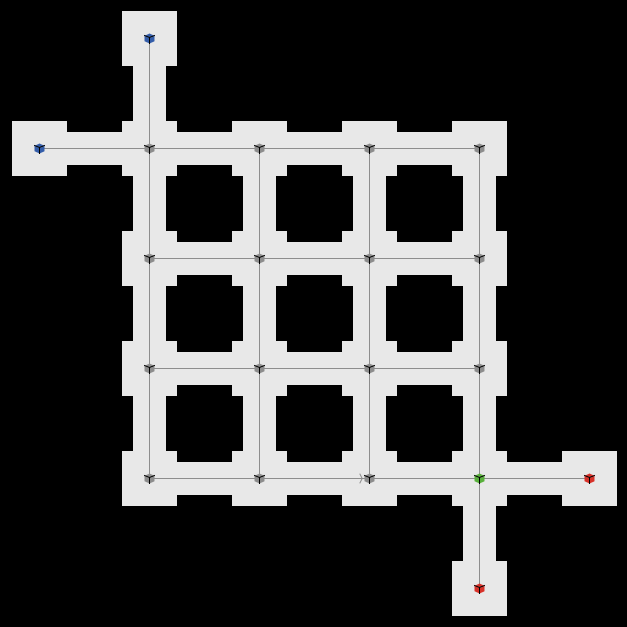
\includegraphics[width=\textwidth,height=\textheight,keepaspectratio]{images/ambiente-screen.png}
\caption{Esempio di ambiente generato. In questo caso i beacons di ingresso sono di colore blu e i beacons di uscita di colore rosso.}
\label{fig:ambiente-screen}
\end{figure}
Per i beacons di ingresso e di uscita vengono anche impostati i relativi parametri, ovvero tasso di generazione o eliminazione degli attori e percentuali relative ai behavior da attribuire ad essi. In particolare per gli entry points si imposta anche un limite massimo del numero di attori che possono essere generati.

Grazie a questi parametri il sistema è predisposto per lo studio di simulazioni in ambienti comunicanti, in cui quindi gli attori possono uscire da un ambiente e entrare in un altro. 

\subsection{Behaviors e stato iniziale}
Abbiamo scelto di caratterizzare i behaviors degli attori con un identificatore intero e una lista di nodi di interesse che l'attore deve raggiungere prima di uscire dall'ambiente.

Sono state inoltre inserite due possibili modalità di raggiungimento dei beacons di interesse: ”\texttt{minDistance}” e “\texttt{orderedList}”. Nella prima l'attore punta al nodo più vicino a quello precedentemente raggiunto tra quelli di interesse, nella seconda invece la lista viene rigidamente percorsa rispettandone l'ordine.

Lo stato iniziale del sistema è contenuto in una semplice lista \texttt{initial-state} che viene percorsa da una apposita funzione per la corretta generazione degli attori sui vari nodi.
 
\begin{figure}[htbp]
\centering
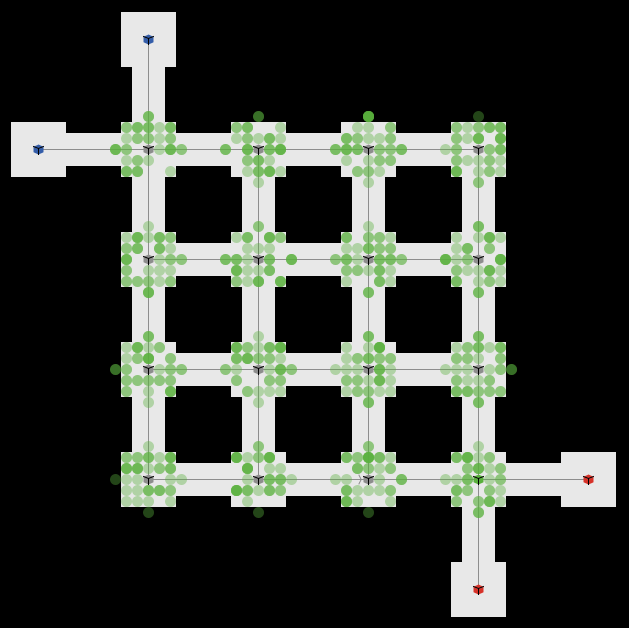
\includegraphics[width=\textwidth,height=\textheight,keepaspectratio]{images/movers-screen.png}
\caption{Esempio di ambiente popolato con attori nello stato iniziale. Gli attori hanno assunto il colore del beacon che hanno come obiettivo, in questo caso abbiamo un unico behavior che ha come interest point il beacon di colore verde.}
\label{fig:movers-screen}
\end{figure}

\section{Librerie usate}
\label{sec:librerie}
La scelta del linguaggio XML è dettata dalla sua diffusione, con lo scopo di ridurre le conoscenze preliminari necessarie per l'utilizzo di questo strumento e per facilitare la sua integrazione con altri componenti.

Per l'analisi del documento XML esistono diverse alternative, tra le quali le più interessanti sono: DOM, SAX e JDOM.

DOM (Document Object Model) è uno standard cross-platform e language-indipendent stabilito dal W3C per la rappresentazione di documenti strutturati, quindi XML, HTML, XHTML, come modelli orientati agli oggetti. Il difetto di questo formato e delle sue API, però, sta nella pesantezza in memoria.

La tecnologia SAX (Simple Api for Xml) rappresenta un'alternativa veloce e potente nel caso in cui si voglia gestire il documento con un approccio event-driven.

JDOM \cite{jdom}, infine, è un formato open-source disegnato appositamente per Java che completa DOM e SAX semplificando la manipolazione dei documenti XML. Questo al contrario delle due alternative non è incluso nel JDK, ma è ampiamente accettato dalla comunità.

Il metodo più rapido e semplice per analizzare un documento XML e costruire un modello JDOM è attraverso le API SAX, che JDOM, grazie alla sua natura open source, può sfruttare.

La API JDOM2 associata al formato, quindi, usa la classe \texttt{SAXBuilder} \cite{sax-builder} per costruire il modello JDOM sotto forma di albero che rispecchia la struttura del documento da cui è stato estratto. 

Per quanto riguarda la parte della scrittura del codice NetLogo, si ha che gran parte del codice che modella la simulazione rimane fissa al variare dei modelli descritti negli XML, quindi abbiamo pensato di mantenere questa in un semplice file di testo che viene letto e integrato con le informazioni contenute negli oggetti Java. Per le operazioni di lettura e scrittura su file abbiamo usato le classi \texttt{BufferedReader} \cite{buffered-reader} e \texttt{PrintWriter} \cite{print-writer} che permettono lettura e scrittura di intere linee di testo.

Lo strumento segue il seguente workflow:
\begin{itemize}
\item analisi del documento XML e costruzione di una rappresentazione della struttura orientata agli oggetti in JDOM attraverso la relativa API;
\item costruzione degli oggetti Java per la rappresentazione della simulazione descritta nel modello JDOM;
\item visita degli oggetti Java e scrittura su file del codice NetLogo che eseguirà la simulazione.
\end{itemize}

\begin{figure}[htbp]
\centering
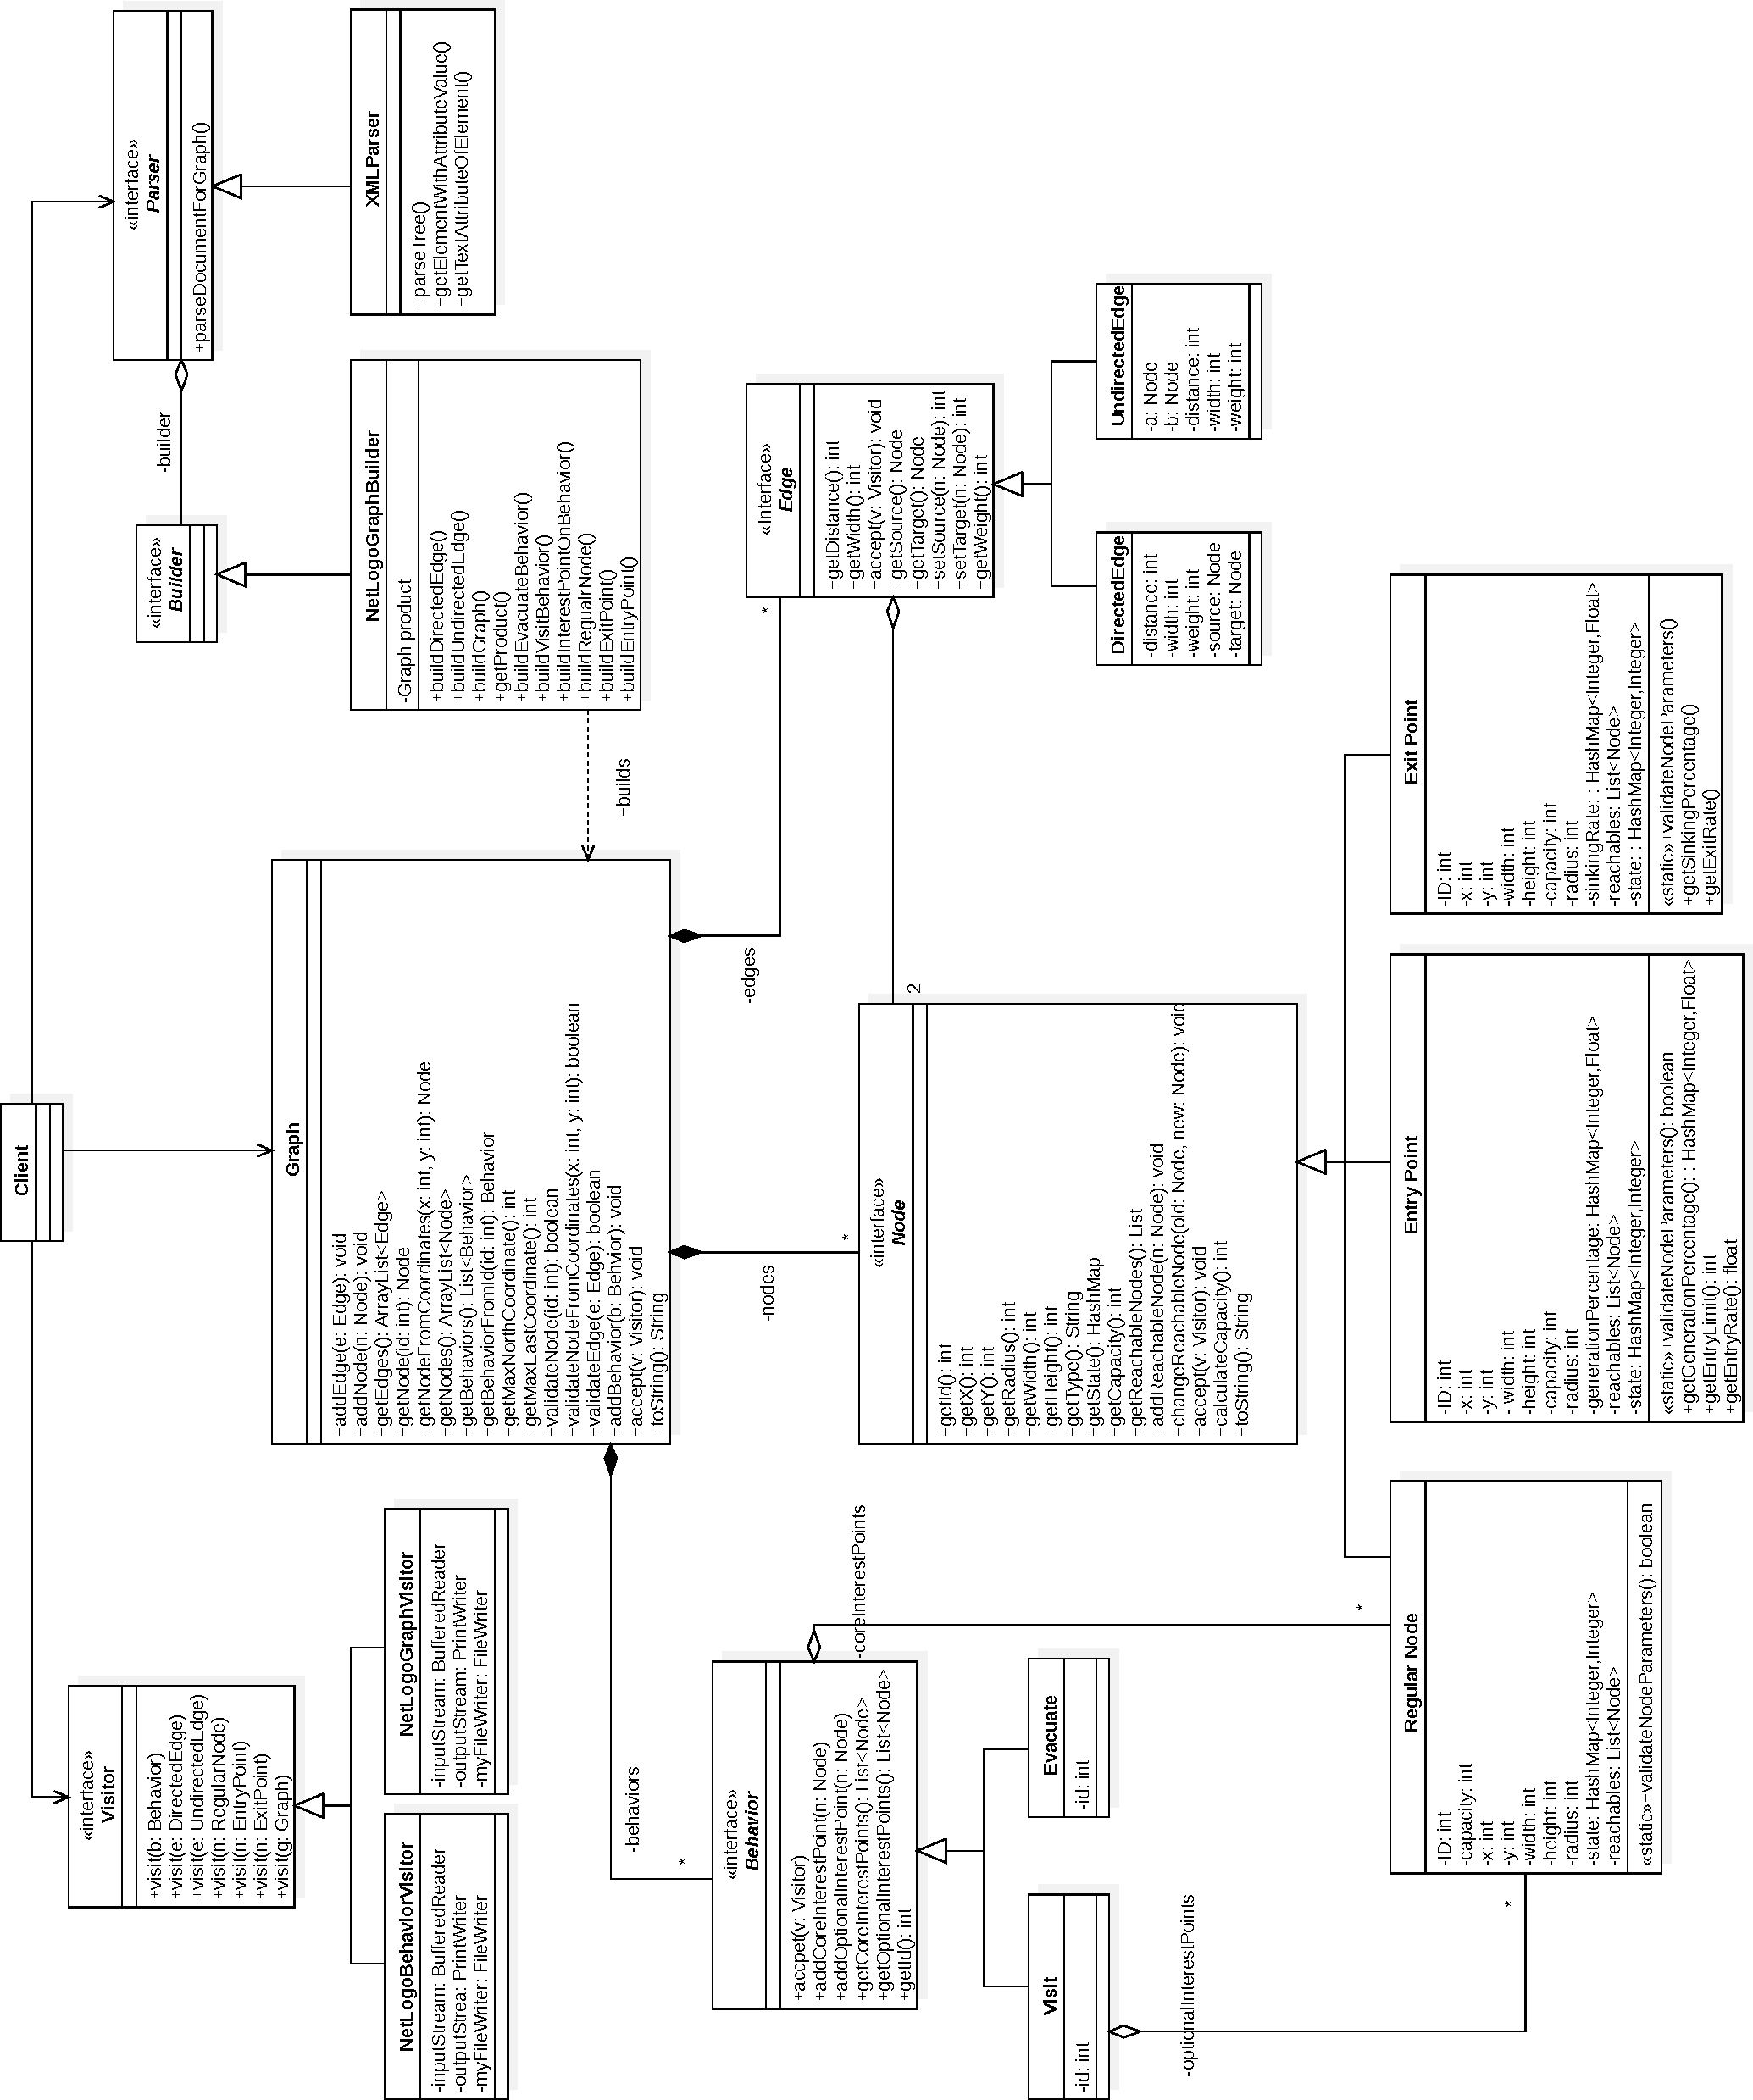
\includegraphics[width=\textwidth,height=\textheight,keepaspectratio]{images/complete-diagram.pdf}
\caption{Classi diagram}
\label{fig:complete-diagram}
\end{figure}

%\chapter{Esperimenti e risultati}

Nella fase di sperimentazione del componente ci siamo posti come obiettivo quello di mettere a confronto la simulazione di un modello monolitico e completo con le simulazioni localizzate su specifiche sezioni in cui quest'ultimo è stato diviso. In particolare abbiamo deciso di confrontare il modello completo con due scenari diversi in cui quest'ultimo è stato diviso in 6 e 12 macro regioni adiacenti.

La mappa usata per gli esperimenti è tratta da un blocco residenziale della città di Firenze, in cui abbiamo cercato di inserire topologie diverse, in modo da rappresentare zone come il centro storico, con strade brevi e strette, e i quartieri delle metropoli moderne, con strade di dimensioni maggiori.

La medesima mappa è stata usata dal gruppo di ricerca del Software Science and Technology Laboratory in \cite{esperimenti-sandro} durante la fase di sperimentazione, in cui, inoltre, si è reso utile il componente sviluppato in questo progetto.

\section{Modello monolitico}
La struttura del modello monolitico è rappresentata in figura X. Lo stato iniziale del sistema è di 10000 agenti distribuiti uniformemente in tutto lo spazio disponibile. Quindi le regioni con maggiore densità di strade saranno popolate anche da un numero maggiore di attori. 

Per avere una stima sufficientemente rappresentativa del tempo di evacuazione di un ambiente è solitamente necessario eseguire almeno 10 simulazioni dello stesso modello. Nel nostro caso il tempo medio ad eseguire una singola simulazione è 55:58 minuti, quindi per ottenere la stima desiderata sono necessarie circa 9:19:40 ore di simulazioni.

Il gruppo di ricerca del STLAB in \cite{esperimenti-sandro} ha usato le simulazioni eseguite su questo modello come riferimento realistico con cui confrontare le approssimazioni generate a partire dai diversi scenari introdotti. Sono state eseguite 8 simulazioni del medesimo modello in modo da avere una buona approssimazione del tempo medio di evacuazione. Attraverso i dati raccolti i ricercatori hanno generato il grafico in Figura X in cui si mostra la ECDF della probabilità di aver evacuato l'ambiente al tempo t.

\section{Scenari con macro regioni}

Nei due scenari la mappa è suddivisa in 6 e 12 sezioni indipendenti in cui i punti di uscita sono punti di connessione con le regioni confinanti. Per ognuna di queste zone sono eseguite simulazioni con 3 diversi stati iniziali, ovvero con densità di affollamento alta, media e bassa. 

Abbiamo inoltre lanciato le simulazioni in due modalità diverse: rigenerativa e non rigenerativa o transitiva (transiente?). La modalità transitiva è la più semplice e rapida delle due, infatti non prevede la generazione di alcun attore, quindi si registrano solo i dati relativi agli agenti che costituiscono lo stato iniziale della regione. La modalità rigenerativa, invece, consiste nel mantenere costante la densità di attori all'interno della regione generando un nuovo agente ogni volta che qualcuno raggiunge l'uscita ed eseguendo il modello per un numero prefissato di unità temporali. In questo modo si ottengono informazioni sui tempi di transizione del sistema che si trova in uno stato stabile di affollamento.

In \cite{esperimenti-sandro} i tempi di transizione ottenuti dai modelli rigenerativi sono usati per calcolare le probabilità di transizione della Catena di Markov che astrae il comportamento dell'attore attraverso le varie regioni come spiegato nella Sezione \ref{sec:approccio-gerarchico}.



\section{Risultati}

Dagli esperimenti condotti abbiamo estratto i tempi necessari ad eseguire un numero consistente di simulazioni dalle quale estrarre i tempi di transizione dei vari attori. Nella tabella X sono confrontati il modello monolitico con 

 
%\chapter{Conclusioni e sviluppi futuri}
Abbiamo mostrato il funzionamento del componente Java sviluppato e illustrato il contesto in cui questo si è rivelato utile semplificando il processo di costruzione ed esecuzione delle simulazioni di folle. Gli esperimenti condotti ci hanno permesso di verificare che i suoi comportamenti rispettassero sempre le attese. 

Nei modelli generati dal componente ci siamo focalizzati sull'aspetto fisico degli attori, modellando gli obiettivi che questi avevano all'interno dell'ambiente. Come lavoro futuro, quindi, sarebbe interessante estendere la logica rappresentativa dei comportamenti degli attori, includendo aspetti sociali come altruismo e conformismo, in modo da rendere i modelli generati ancora più vicini alla realtà. 

Un ulteriore sviluppo di questo progetto è sicuramente l'inclusione di nuovi parser in grado di analizzare formati diversi dall'XML, come ad esempio il CSV, e l'implementazione di una interfaccia, estendendo quindi i contesti in cui questo framework potrebbe rendersi utile e semplificandone l'utilizzo.

\include{files/bibliography}

\addcontentsline{toc}{chapter}{Bibliografia}
\bibliographystyle{plain}
\bibliography{files/bibliography}

%\chapter{Ringraziamenti}

Ringrazio il professor Enrico Vicario per avermi dato la possibilità di svolgere questo lavoro di tesi su un argomento molto interessante. Un particolare ringraziamento va al mio co-relatore Sandro Mehic che con molta pazienza e costanza mi ha aiutato e insegnato tantissimo in questi mesi.

Ringrazio prima tra tutti mia sorella che mi ha sempre sostenuto e incoraggiato nei momenti più difficili diventando il mio punto di riferimento e facendo di me quello che sono oggi. Ringrazio mia madre e mio padre che con tantissimi sacrifici mi hanno permesso di raggiungere questo traguardo importantissimo. Un grazie di cuore va anche a Bernardo che non si è mai arreso nel darmi consigli e nello spingermi a provare cose nuove. Alla mia famiglia dedico tutto ciò che ho realizzato fino ad oggi, senza il loro sostegno non ce l'avrei mai fatta.



\end{document}